\documentclass[landscape,final,a0paper,fontscale=0.285]{baposter}

\usepackage{calc}
\usepackage{graphicx}
\usepackage{amsmath}
\usepackage{amssymb}
\usepackage{relsize}
\usepackage{multirow}
\usepackage{rotating}
\usepackage{bm}
\usepackage{url}
\usepackage[font=small,labelfont=bf, justification=justified,singlelinecheck=false]{caption}% newly added by me
\usepackage{color, colortbl}
\usepackage{graphicx}
\usepackage{multicol}
\usepackage{palatino}

%\newcommand{\captionfont}{\footnotesize}

\graphicspath{{images/}{../images/}}
\usetikzlibrary{calc}

\newcommand{\SET}[1]  {\ensuremath{\mathcal{#1}}}
\newcommand{\MAT}[1]  {\ensuremath{\boldsymbol{#1}}}
\newcommand{\VEC}[1]  {\ensuremath{\boldsymbol{#1}}}
\newcommand{\Video}{\SET{V}}
\newcommand{\video}{\VEC{f}}
\newcommand{\track}{x}
\newcommand{\Track}{\SET T}
\newcommand{\LMs}{\SET L}
\newcommand{\lm}{l}
\newcommand{\PosE}{\SET P}
\newcommand{\posE}{\VEC p}
\newcommand{\negE}{\VEC n}
\newcommand{\NegE}{\SET N}
\newcommand{\Occluded}{\SET O}
\newcommand{\occluded}{o}

%%%%%%%%%%%%%%%%%%%%%%%%%%%%%%%%%%%%%%%%%%%%%%%%%%%%%%%%%%%%%%%%%%%%%%%%%%%%%%%%
%%%% Some math symbols used in the text
%%%%%%%%%%%%%%%%%%%%%%%%%%%%%%%%%%%%%%%%%%%%%%%%%%%%%%%%%%%%%%%%%%%%%%%%%%%%%%%%

%%%%%%%%%%%%%%%%%%%%%%%%%%%%%%%%%%%%%%%%%%%%%%%%%%%%%%%%%%%%%%%%%%%%%%%%%%%%%%%%
% Multicol Settings
%%%%%%%%%%%%%%%%%%%%%%%%%%%%%%%%%%%%%%%%%%%%%%%%%%%%%%%%%%%%%%%%%%%%%%%%%%%%%%%%
\setlength{\columnsep}{1.5em}
\setlength{\columnseprule}{0mm}

%%%%%%%%%%%%%%%%%%%%%%%%%%%%%%%%%%%%%%%%%%%%%%%%%%%%%%%%%%%%%%%%%%%%%%%%%%%%%%%%
% Save space in lists. Use this after the opening of the list
%%%%%%%%%%%%%%%%%%%%%%%%%%%%%%%%%%%%%%%%%%%%%%%%%%%%%%%%%%%%%%%%%%%%%%%%%%%%%%%%
\newcommand{\compresslist}{%
\setlength{\itemsep}{1pt}%
\setlength{\parskip}{0pt}%
\setlength{\parsep}{0pt}%
}

%%%%%%%%%%%%%%%%%%%%%%%%%%%%%%%%%%%%%%%%%%%%%%%%%%%%%%%%%%%%%%%%%%%%%%%%%%%%%%
%%% Begin of Document
%%%%%%%%%%%%%%%%%%%%%%%%%%%%%%%%%%%%%%%%%%%%%%%%%%%%%%%%%%%%%%%%%%%%%%%%%%%%%%

\begin{document}

%%%%%%%%%%%%%%%%%%%%%%%%%%%%%%%%%%%%%%%%%%%%%%%%%%%%%%%%%%%%%%%%%%%%%%%%%%%%%%
%%% Here starts the poster
%%%---------------------------------------------------------------------------
%%% Format it to your taste with the options
%%%%%%%%%%%%%%%%%%%%%%%%%%%%%%%%%%%%%%%%%%%%%%%%%%%%%%%%%%%%%%%%%%%%%%%%%%%%%%
% Define some colors

%\definecolor{lightblue}{cmyk}{0.83,0.24,0,0.12}
\definecolor{lightblue}{rgb}{0.145,0.6666,1}

\hyphenation{resolution occlusions}
%%
\begin{poster}%
  % Poster Options
  {
  % Show grid to help with alignment
  grid=false,
  % Column spacing
  colspacing=1em,
  % Color style
  bgColorOne=white,
  bgColorTwo=white,
  borderColor=lightblue,
  headerColorOne=black,
  headerColorTwo=lightblue,
  headerFontColor=white,
  boxColorOne=white,
  boxColorTwo=lightblue,
  % Format of textbox
  textborder=roundedleft,
  % Format of text header
  eyecatcher=true,
  headerborder=none,
  headerheight=0.08\textheight,
%  textfont=\sc, An example of changing the text font
  headershape=roundedright,
  headershade=shadelr,
  headerfont=\Large\bf\textsc, %Sans Serif
  textfont={\setlength{\parindent}{1.5em}},
  boxshade=plain,
%  background=shade-tb,
  background=plain,
  linewidth=2pt
  }
  % Eye Catcher
  {
\includegraphics[height=7em]{images/SACON.png}} 
  % Title
  %{\includegraphics[height=5em]{images/graph_occluded.pdf}} 
  % Title
  {\sf\Large\textbf{Regional temperature variability in the Western Ghats}\vspace{0.1em}}
  % Authors
  {\sf\small\textit{\ Nishadh K A and Azeez P A \\Environmental Impact Assessment Division, Salim Ali Centre for Ornithology and Natural History(SACON)\\ Anaikatty (PO), Coimbatore - 641108, Tamil Nadu}}
  % University logo
  %{% The makebox allows the title to flow into the logo, this is a hack because of the L shaped logo.
   % 
\includegraphics[height=5.0cm]{images/SACON}
  %}
  
%%%%%%%%%%%%%%%%%%%%%%%%%%%%%%%%%%%%%%%%%%%%%%%%%%%%%%%%%%%%%%%%%%%%%%%%%%%%%%
%%% Now define the boxes that make up the poster
%%%---------------------------------------------------------------------------
%%% Each box has a name and can be placed absolutely or relatively.
%%% The only inconvenience is that you can only specify a relative position 
%%% towards an already declared box. So if you have a box attached to the 
%%% bottom, one to the top and a third one which should be in between, you 
%%% have to specify the top and bottom boxes before you specify the middle 
%%% box.
%%%%%%%%%%%%%%%%%%%%%%%%%%%%%%%%%%%%%%%%%%%%%%%%%%%%%%%%%%%%%%%%%%%%%%%%%%%%%%
    %
    % A coloured circle useful as a bullet with an adjustably strong filling
    \newcommand{\colouredcircle}{%
      \tikz{\useasboundingbox (-0.2em,-0.32em) rectangle(0.2em,0.32em); \draw[draw=black,fill=lightblue,line width=0.03em] (0,0) circle(0.18em);}}

%%%%%%%%%%%%%%%%%%%%%%%%%%%%%%%%%%%%%%%%%%%%%%%%%%%%%%%%%%%%%%%%%%%%%%%%%%%%%%
  \headerbox{Introduction}{name=introduction,column=0,row=0, span=2}{
%%%%%%%%%%%%%%%%%%%%%%%%%%%%%%%%%%%%%%%%%%%%%%%%%%%%%%%%%%%%%%%%%%%%%%%%%%%%%%
  \begin {description}
  \footnotesize
\item [Scale variant] mode and impact of climate change necessitates local to regional level assessment.
\item [Surface air temperature] records provide invaluable information for those assessments but have certain limitations because of sparse observations.  
\item [Limitations] of sparse regional temperature observations can be addressed by improved averaging and statistical models such as Berkley averaging process (Rhode).  
\item [Present study] assess the long term regional temperature variability in the Western Ghats, its station wise temperature trend, temperature anomaly and month wise regional average temperature trend.
\item [Importance] of these assessments is that it can give understandings on extent and trend of temperature variability, a diagnosis for climate change, thus have great importance in understanding and devising appropriate adaptation strategy towards climate change.
\end {description}
   \vspace{0.1em}
 }

%%%%%%%%%%%%%%%%%%%%%%%%%%%%%%%%%%%%%%%%%%%%%%%%%%%%%%%%%%%%%%%%%%%%%%%%%%%%%%
 \headerbox{Methods}{name=methods,column=0,row=0,below=introduction, span=2}{
%%%%%%%%%%%%%%%%%%%%%%%%%%%%%%%%%%%%%%%%%%%%%%%%%%%%%%%%%%%%%%%%%%%%%%%%%%%%%%
\footnotesize  Regional temperature variability assessment study comprised of three steps
\noindent \begin{multicols}{3}
\noindent \begin{minipage}{\linewidth}
\textbf{Data Collection}
\scriptsize \begin{enumerate}
      \item Western Ghats region was considered as the boundaries of 44 districts criss crossed by 1,600 km long western ghats mountain chain.
      \item Temperature data of the stations situated within this region was extracted from Berkley earth surface temperature study dataset.
      \item Temperature Data comprised of Monthly average temperature (TAVG), monthly maximum (TMAX) and minimum temperature (TMIN), dated from 1835 for TAVG and 1981 for TMAX and TMIN to 2011.
   \end{enumerate}
\end{minipage}
\begin{minipage}{\linewidth}
\centering
%\vspace{1 cm}
%\hspace{3 cm}
\label{tab:name}
\begin{tabular}{@{}c@{ }}
    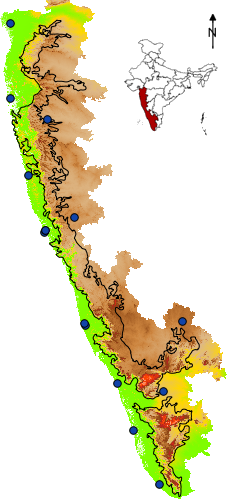
\includegraphics[width=3cm,height=4.6cm]{WG_stat.png}                     
 \end{tabular}
\captionof{figure}{\scriptsize Stations locations}
\end{minipage}

\noindent\begin{minipage}{\linewidth}
\footnotesize
\textbf{Data validation}
\scriptsize \begin{enumerate}
\item Long term data necessitates the need of data validation of any spurious change-points in observations.
\item Under this process the data will be subjected to homogenization testing and adjustment if necessary.
\item Penalized maximal  F test (Wang et al. 2008) is used to test the homogeneity in the data.
\item It tests the linear trend in data period with iterative identification of mean shifts (change points) using annual cycle, linear trend, and lag-1 autocorrelation of the base time series data. 
\item Station was selected if the data was available for more than 10 year observations.
Thus 17 stations data were selected for analysis out of the 26 stations in the Western Ghats region. 
      \end{enumerate}
\footnotesize\textbf{Trend Analysis}
\scriptsize\begin{enumerate}
      \item Comprised of Regional average determination and statistical testing of observed trend.
      \item Modified Berkley local averaging process was used (Tamino 2012); it computes local average based on equal weighting and offset method.
\end{enumerate}
\end {minipage}
\noindent\begin {minipage}{\linewidth}
\scriptsize
\vspace{5 mm}
      \small \begin{enumerate}
      \scriptsize
      \setcounter{enumi}{2}
      \item The averaging is computed based on equation
      \begin{equation*}  
\gamma _{\textit k}= (\frac{1}{N}_{\textit k}) \sum _{stations}(y_{\textit j}(t_{\textit k}) - \mu _{\textit j})
\end{equation*}
      \item The offset is computed based on equation 
      \begin{equation*}
\mu _{\textit j}= (\frac{1}{N}_{\textit j}) \sum _{times}(y_{\textit j}(t_{\textit k}) - \gamma _{\textit k})
\end{equation*}
where ${{N}_{\textit k}}$ is number of stations with data at time ${t_{\textit k}}$\\ ${{N}_{\textit j}}$ is number of time points for which station ${\textit j}$ has data,\\ ${(y_{\textit j}(t_{\textit k})}$ is the data record for station ${\textit j}$.
      \item The trend in regional average time series were analyzed using non parametric Mann-Kendall rank statistics ($\tau$), it is based on equation.  
     \begin{equation*}
\tau_{\textit t}= 0 \pm {\textit t}_{\textit g}\sqrt {4{\textbf N+10}/9 {\textbf N}(\textbf N} -1)
\end{equation*}
where $\tau_{\textit t}$ with probability value ${\textit t}_{\textit g}$ gives siginificance test for observed trend.
\item Temperature anomaly was calculated for TAVG of criteria stations having full year data during the period 1961-1990. 
\end{enumerate}
\end{minipage}    
\end{multicols}
   \vspace{0.1em}
  }
 %%%%%%%%%%%%%%%%%%%%%%%%%%%%%%%%%%%%%%%%%%%%%%%%%%%%%%%%%%%%%%%%%%%%%%%%%%%%%% 
\headerbox{results}{name=results1,column=2,row=0, span =2}{
 %%%%%%%%%%%%%%%%%%%%%%%%%%%%%%%%%%%%%%%%%%%%%%%%%%%%%%%%%%%%%%%%%%%%%%%%%%%%%%
\noindent\begin{multicols}{2}  
\tiny
\noindent\begin{minipage}{\linewidth}
\centering
\captionof{table}{\scriptsize Stationwise temperature trend in the Western ghats region}
\label{tab:name}
%\rowcolors{2}{green}{pink}
\noindent
\definecolor {lightgray}{gray}{0.95}
\definecolor {gray}{RGB}{128,128,128}
\begin{tabular}{ccccc}\rowcolor{lightgray}
   STATIONS&& TMAX & TMIN & TAVG\\
\multicolumn{1}{>{\columncolor{white}}l}{}&Average($^\circ$ C)&31.6$\pm$1.12&18.1$\pm$1.21&27.4$\pm$0.80 \\ \rowcolor{lightgray} 
\multicolumn{1}{>{\columncolor{white}}l}{\multirow{-3}{*}{SURAT}}&$\tau$&0.013&0.032&0.028\\
\multicolumn{1}{>{\columncolor{lightgray}}l}{}&Average($^\circ$ C)&31.9$\pm$1.03&22.6$\pm$0.85&27.1$\pm$0.85 \\ \rowcolor{lightgray} 
\multicolumn{1}{>{\columncolor{lightgray}}l}{\multirow{-3}{*}{BOMBAY/SANTACRUZ}}&$\tau$&0.338**&0&0.288**\\
\multicolumn{1}{>{\columncolor{white}}l}{}&Average($^\circ$ C)&31.7$\pm$0.82&23.9$\pm$0.73&27.3$\pm$0.75 \\ \rowcolor{lightgray} 
\multicolumn{1}{>{\columncolor{white}}l}{\multirow{-3}{*}{BOMBAY / COLA}}&$\tau$&0.062&0.217**&0.283**\\
\multicolumn{1}{>{\columncolor{lightgray}}l}{}&Average($^\circ$ C)&31.5$\pm$1.08&18.0$\pm$1.56&24.9$\pm$0.91 \\ \rowcolor{lightgray} 
\multicolumn{1}{>{\columncolor{lightgray}}l}{\multirow{-3}{*}{PUNE}}&$\tau$&0.185**&0&-0.04**\\
\multicolumn{1}{>{\columncolor{white}}l}{}&Average($^\circ$ C)&30.1$\pm$0.87&22.2$\pm$0.81&26.8$\pm$0.67 \\ \rowcolor{lightgray} 
\multicolumn{1}{>{\columncolor{white}}l}{\multirow{-3}{*}{RATNAGIRI}}&$\tau$&0.212**&-0.13**&0.03\\
\multicolumn{1}{>{\columncolor{lightgray}}l}{}&Average($^\circ$ C)&30.2$\pm$0.96&18.4$\pm$1.04&24.3$\pm$0.67 \\ \rowcolor{lightgray} 
\multicolumn{1}{>{\columncolor{lightgray}}l}{\multirow{-3}{*}{BELGAUM/SAMBRA}}&$\tau$&0.241**&-0.08**&0.058\\
\multicolumn{1}{>{\columncolor{white}}l}{}&Average($^\circ$ C)&-&-&24.2$\pm$0.84 \\ \rowcolor{lightgray} 
\multicolumn{1}{>{\columncolor{white}}l}{\multirow{-3}{*}{BELGAUM}}&$\tau$&&&0.342**\\
\multicolumn{1}{>{\columncolor{lightgray}}l}{}&Average($^\circ$ C)&31.6$\pm$0.79&23.4$\pm$0.75&27.4$\pm$0.66 \\ \rowcolor{lightgray} 
\multicolumn{1}{>{\columncolor{lightgray}}l}{\multirow{-3}{*}{GOA/PANJI}}&$\tau$&0.241**&-0.01&0.222**\\
\multicolumn{1}{>{\columncolor{white}}l}{}&Average($^\circ$ C)&31.5$\pm$0.85&23.1$\pm$1.13&27.3$\pm$0.84 \\ \rowcolor{lightgray} 
\multicolumn{1}{>{\columncolor{white}}l}{\multirow{-3}{*}{NOVA GOA}}&$\tau$&-0.30**&-0.09**&-0.23**\\
\multicolumn{1}{>{\columncolor{lightgray}}l}{}&Average($^\circ$ C)&29.7$\pm$0.84&23.7$\pm$0.79&26.7$\pm$0.72 \\ \rowcolor{lightgray} 
\multicolumn{1}{>{\columncolor{lightgray}}l}{\multirow{-3}{*}{MARMAGAO}}&$\tau$&-0.14**&-0.07**&-0.11**\\
\multicolumn{1}{>{\columncolor{white}}l}{}&Average($^\circ$ C)&29.5$\pm$0.89&19.1$\pm$0.68&23.9$\pm$0.71 \\ \rowcolor{lightgray} 
\multicolumn{1}{>{\columncolor{white}}l}{\multirow{-3}{*}{BANGALORE}}&$\tau$&0.196**& 0.22**&0.267**\\
\multicolumn{1}{>{\columncolor{lightgray}}l}{}&Average($^\circ$ C)&31.7$\pm$0.73&23.0$\pm$0.6&27.0$\pm$0.58 \\ \rowcolor{lightgray} 
\multicolumn{1}{>{\columncolor{lightgray}}l}{\multirow{-3}{*}{MANGALORE/BAJPE}}&$\tau$&0.217**&-0.04&0.201**\\
\multicolumn{1}{>{\columncolor{white}}l}{}&Average($^\circ$ C)&30.5$\pm$0.68&23.5$\pm$0.67&27.0$\pm$0.61 \\ \rowcolor{lightgray} 
\multicolumn{1}{>{\columncolor{white}}l}{\multirow{-3}{*}{MANGALORE}}&$\tau$& 0.057*&0.124**&0.118**\\
\multicolumn{1}{>{\columncolor{lightgray}}l}{}&Average($^\circ$ C)&31.3$\pm$0.88&24.2$\pm$0.59&27.7$\pm$0.62 \\ \rowcolor{lightgray} 
\multicolumn{1}{>{\columncolor{lightgray}}l}{\multirow{-3}{*}{KOZHIKODE}}&$\tau$&0.499**&0.258**&0.396**\\
\multicolumn{1}{>{\columncolor{white}}l}{}&Average($^\circ$ C)&32.4$\pm$0.94&21.5$\pm$0.65&26.4$\pm$0.71 \\ \rowcolor{lightgray} 
\multicolumn{1}{>{\columncolor{white}}l}{\multirow{-3}{*}{COIMBATORE}}&$\tau$& 0.082*&0.199**&0.156**\\
\multicolumn{1}{>{\columncolor{lightgray}}l}{}&Average($^\circ$ C)&31.1$\pm$0.69&24.2$\pm$0.59&27.3$\pm$0.54 \\ \rowcolor{lightgray} 
\multicolumn{1}{>{\columncolor{lightgray}}l}{\multirow{-3}{*}{FORT COCHIN}}&$\tau$& 0.084*& 0.087*&0.059**\\
\multicolumn{1}{>{\columncolor{white}}l}{}&Average($^\circ$ C)&31.4$\pm$0.89&23.6$\pm$0.47&27.0$\pm$0.68 \\ \rowcolor{lightgray} 
\multicolumn{1}{>{\columncolor{white}}l}{\multirow{-3}{*}{THIRUVANANTHAPURAM}}&$\tau$&0.429**&0.059&0.476**\\
   \end{tabular}
 *- p<0.05, **- p<0.01
\end{minipage}  
\begin{minipage}{\linewidth}
\centering

\label{tab:name}
 \begin{tabular}{@{}c@{ }}
    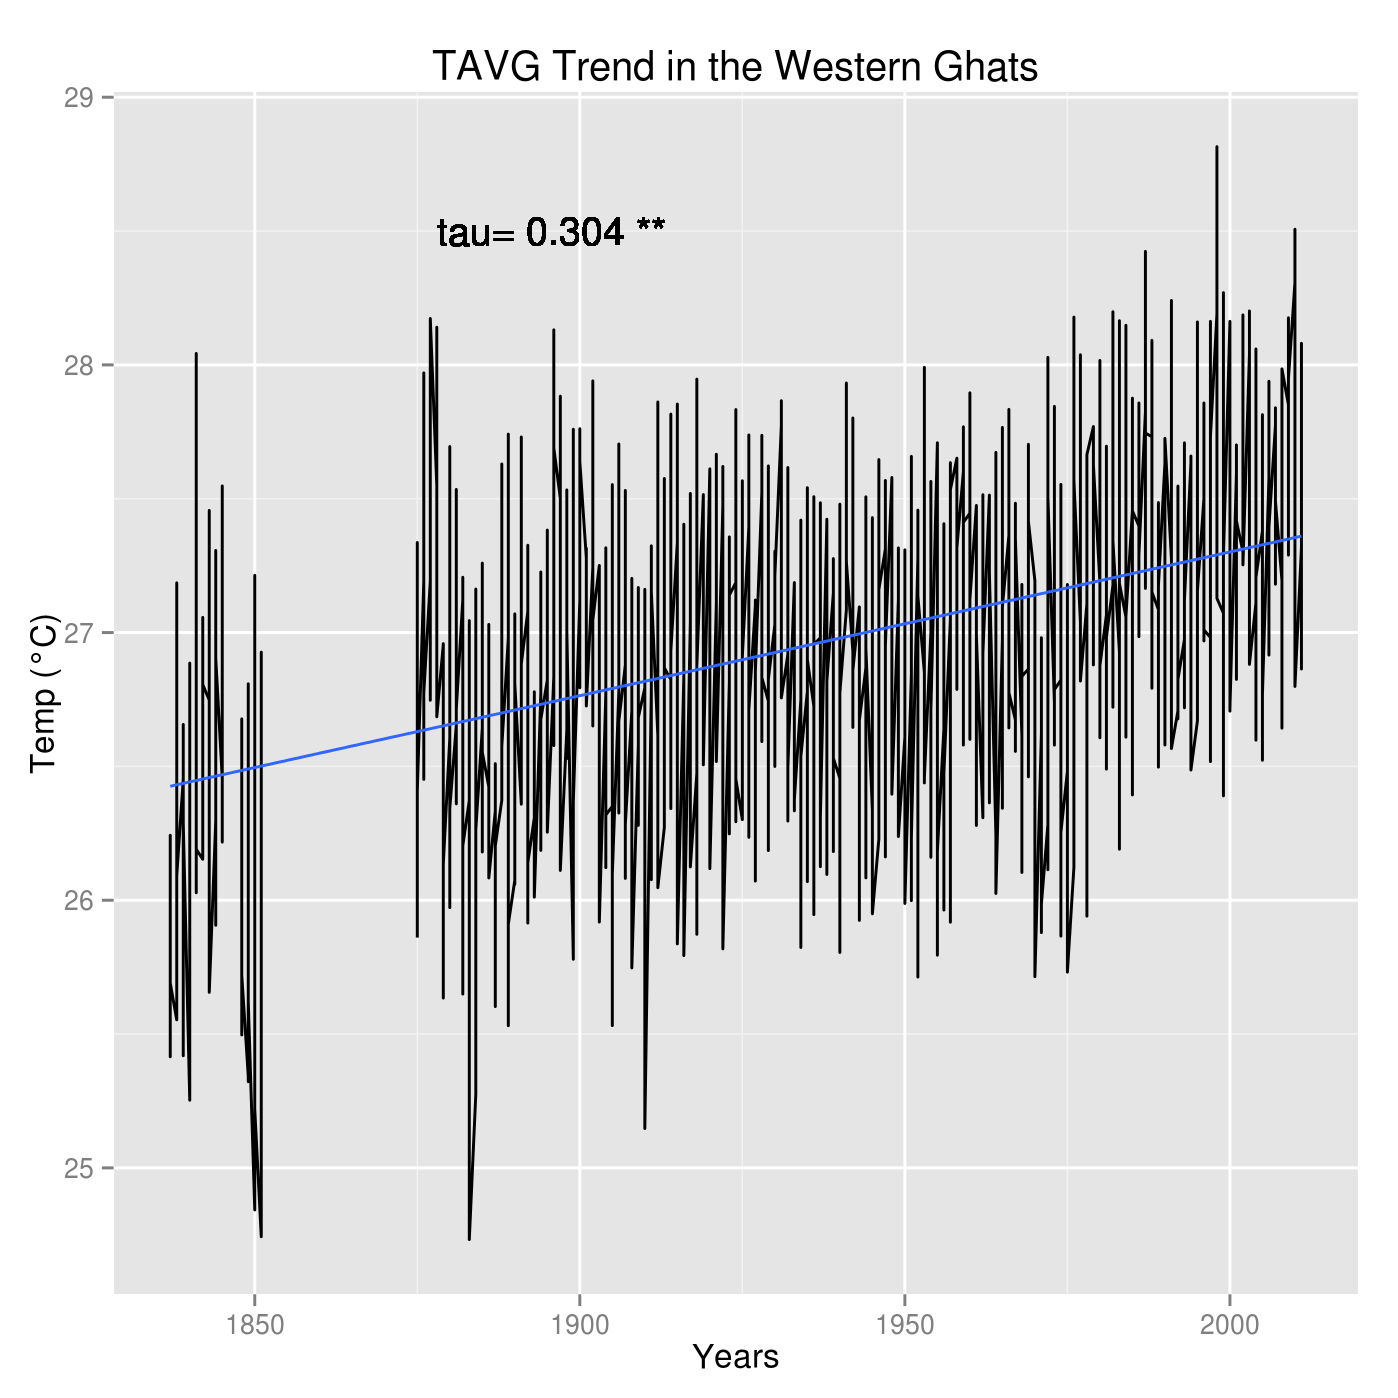
\includegraphics[width=5cm,height=2.7cm]{TAVG.png}\\
    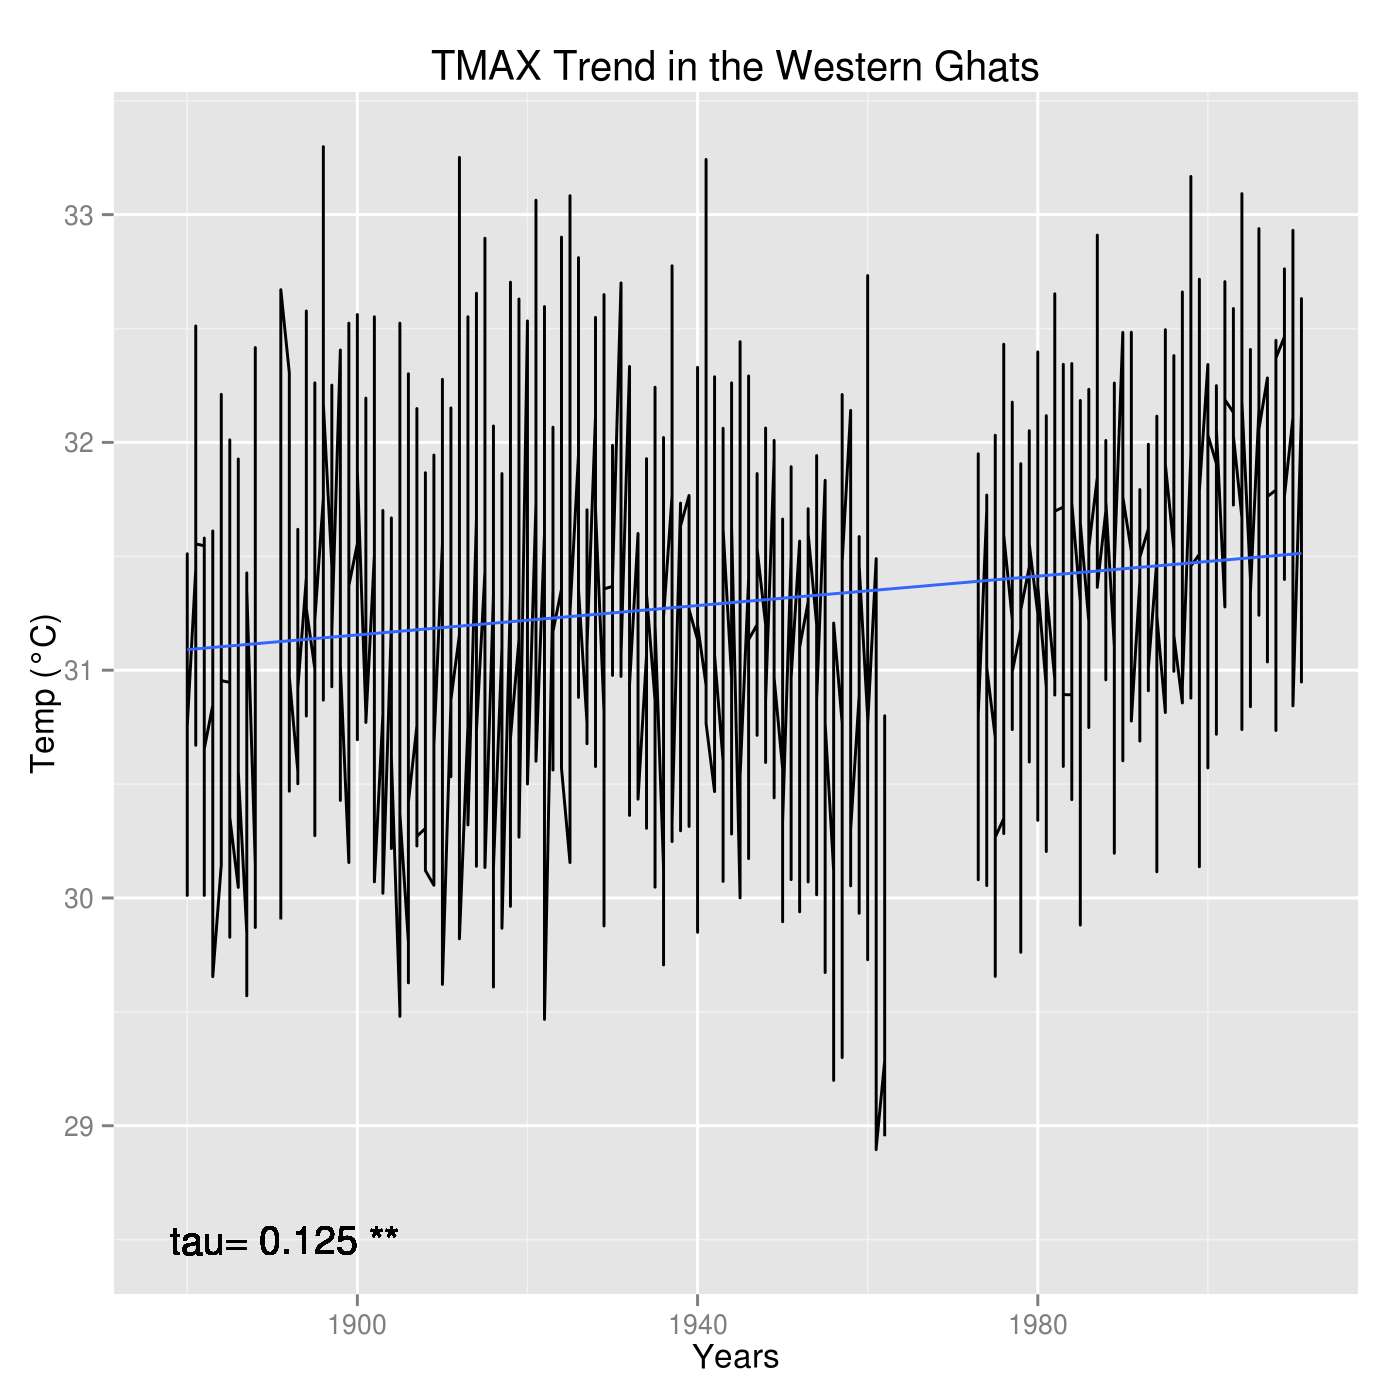
\includegraphics[width=5cm,height=2.7cm]{TMAX.png}\\
    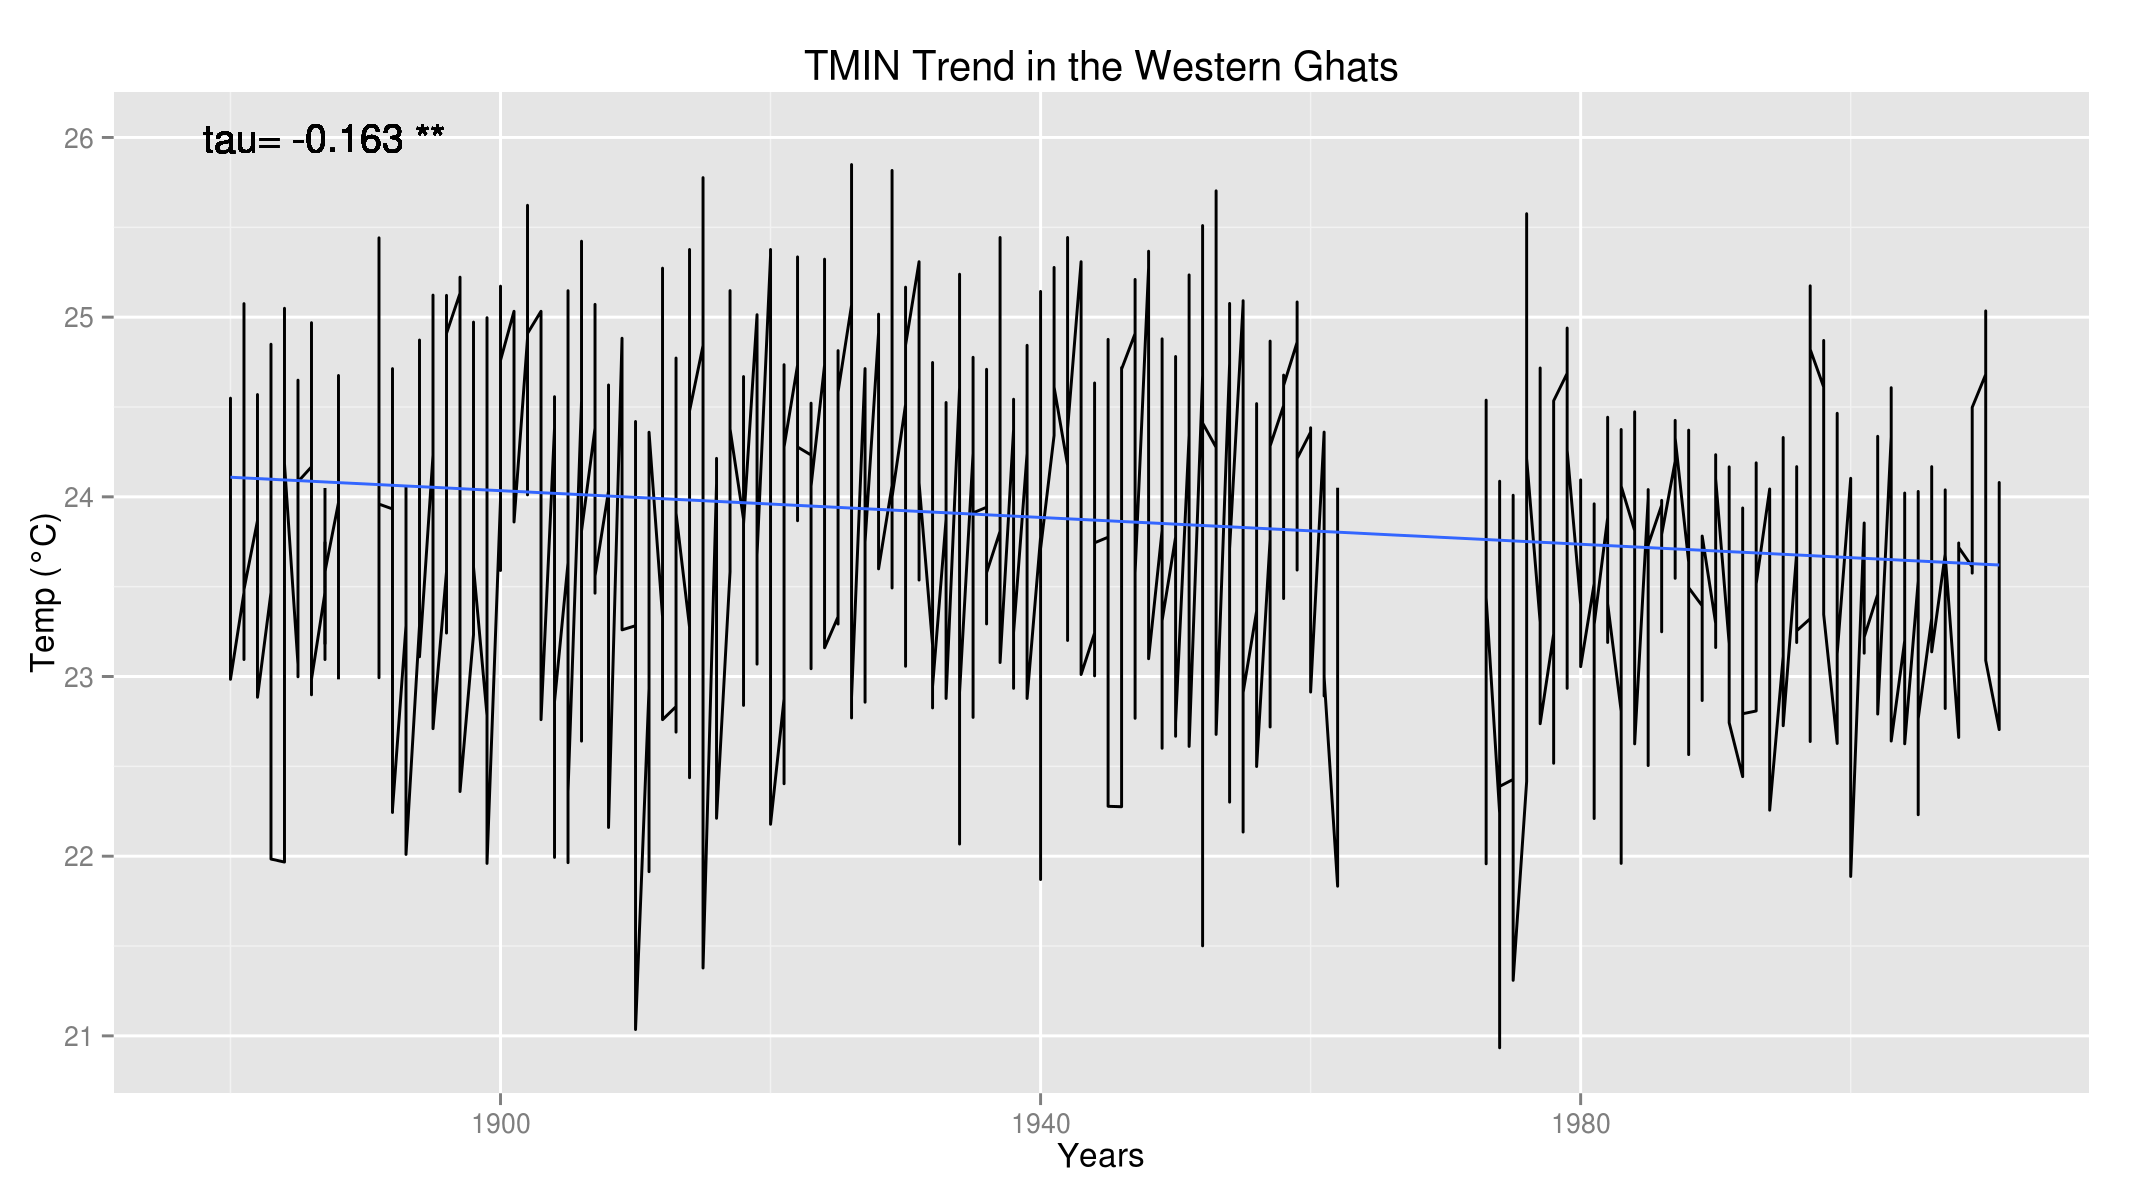
\includegraphics[width=5cm,height=2.7cm]{TMIN.png}\\
                       
  \end{tabular}
\captionof{figure}{\scriptsize Regional average temperature trend in the Western Ghats } 
  \end{minipage} 
\end{multicols}

\noindent\begin{minipage}{\linewidth}
\centering

\label{tab:name}
\noindent\begin{tabular}{@{}c@{}c@{}c@{}c@{}c@{}c@{}}
    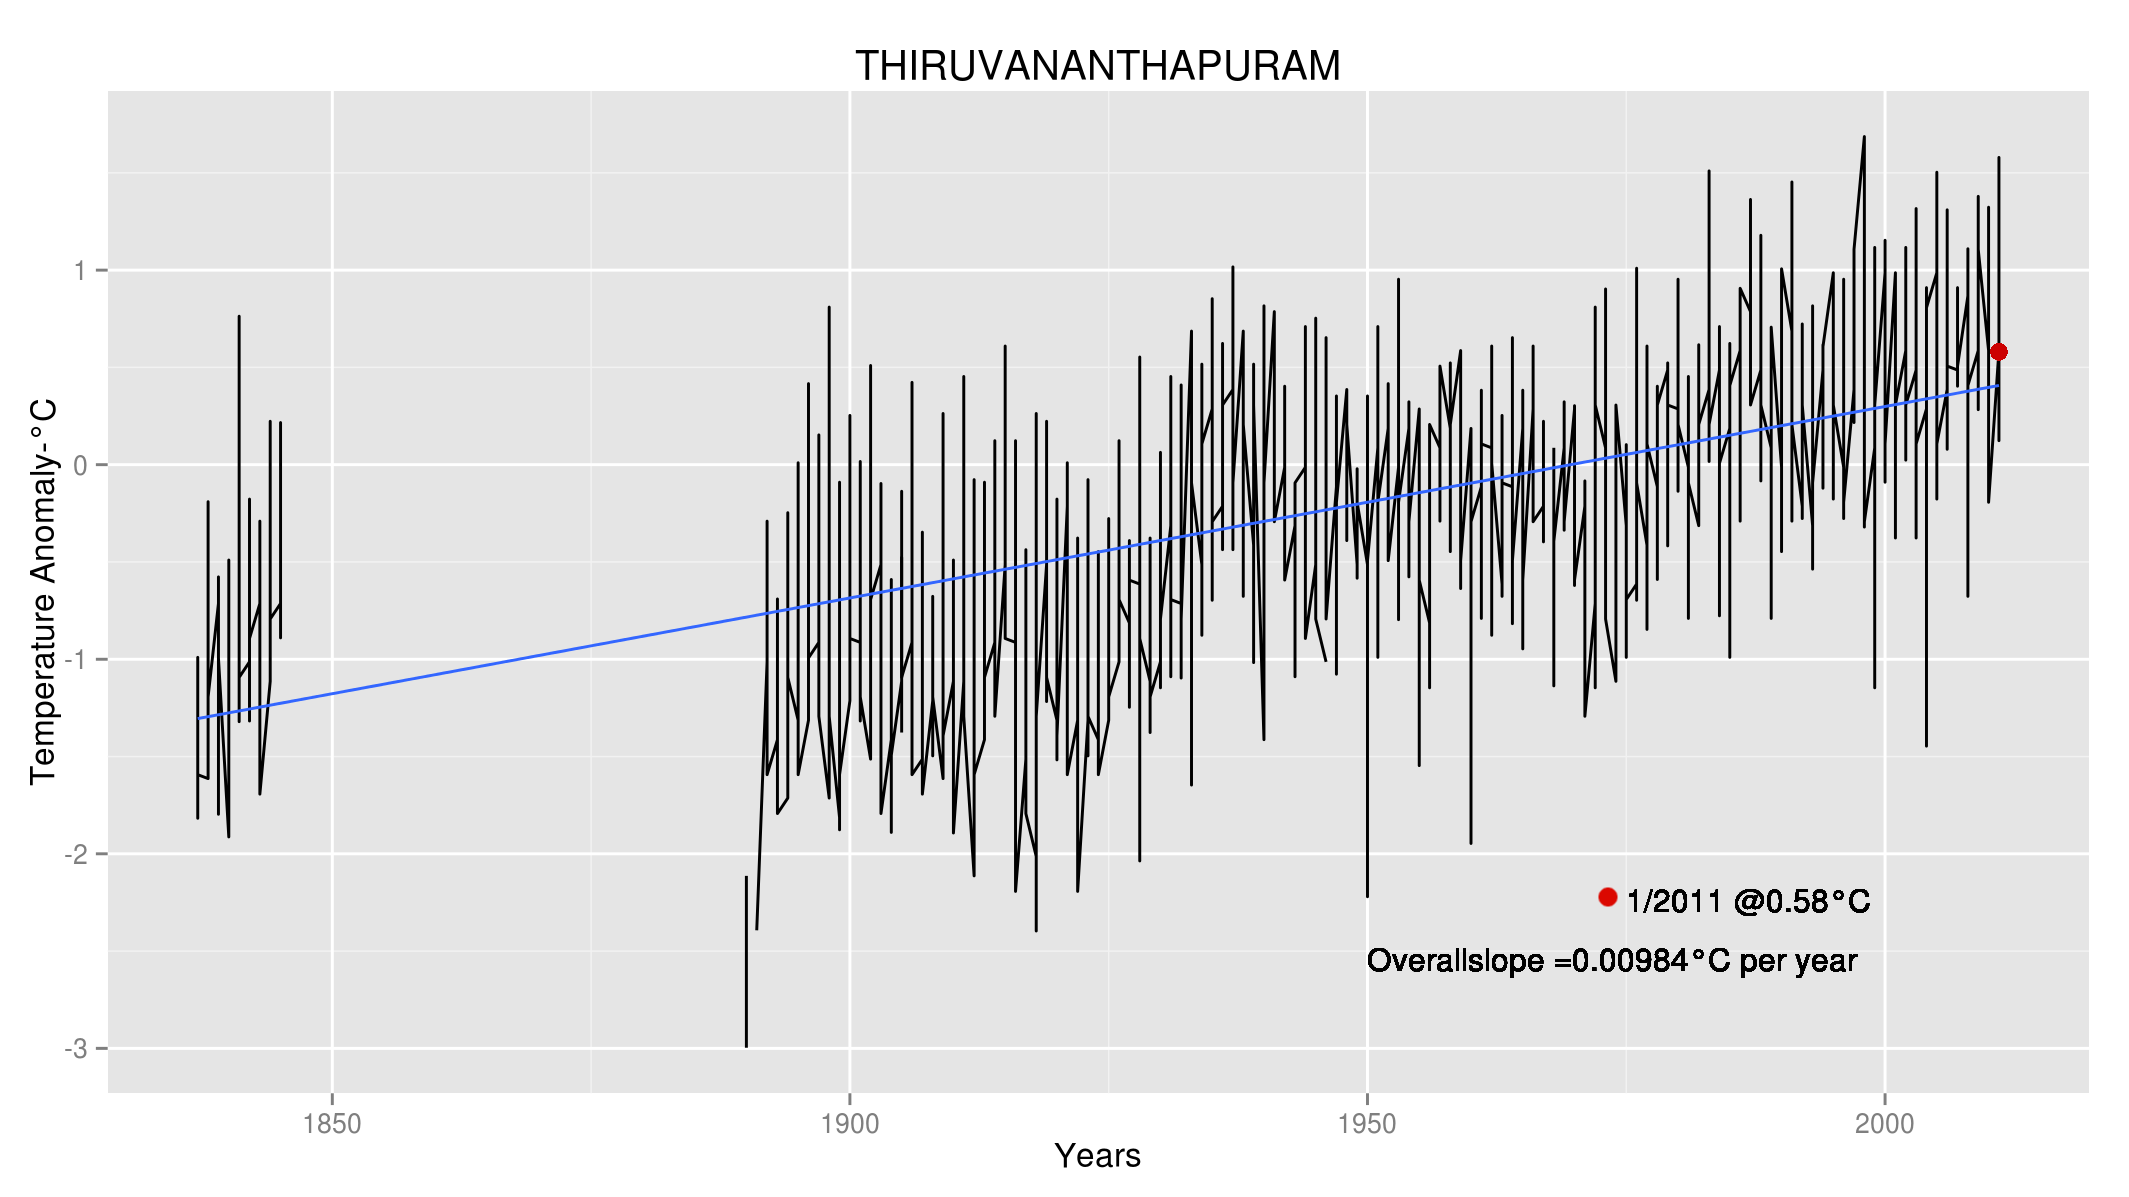
\includegraphics[width=3.2cm,height=3.2cm]{X15075.png}&
	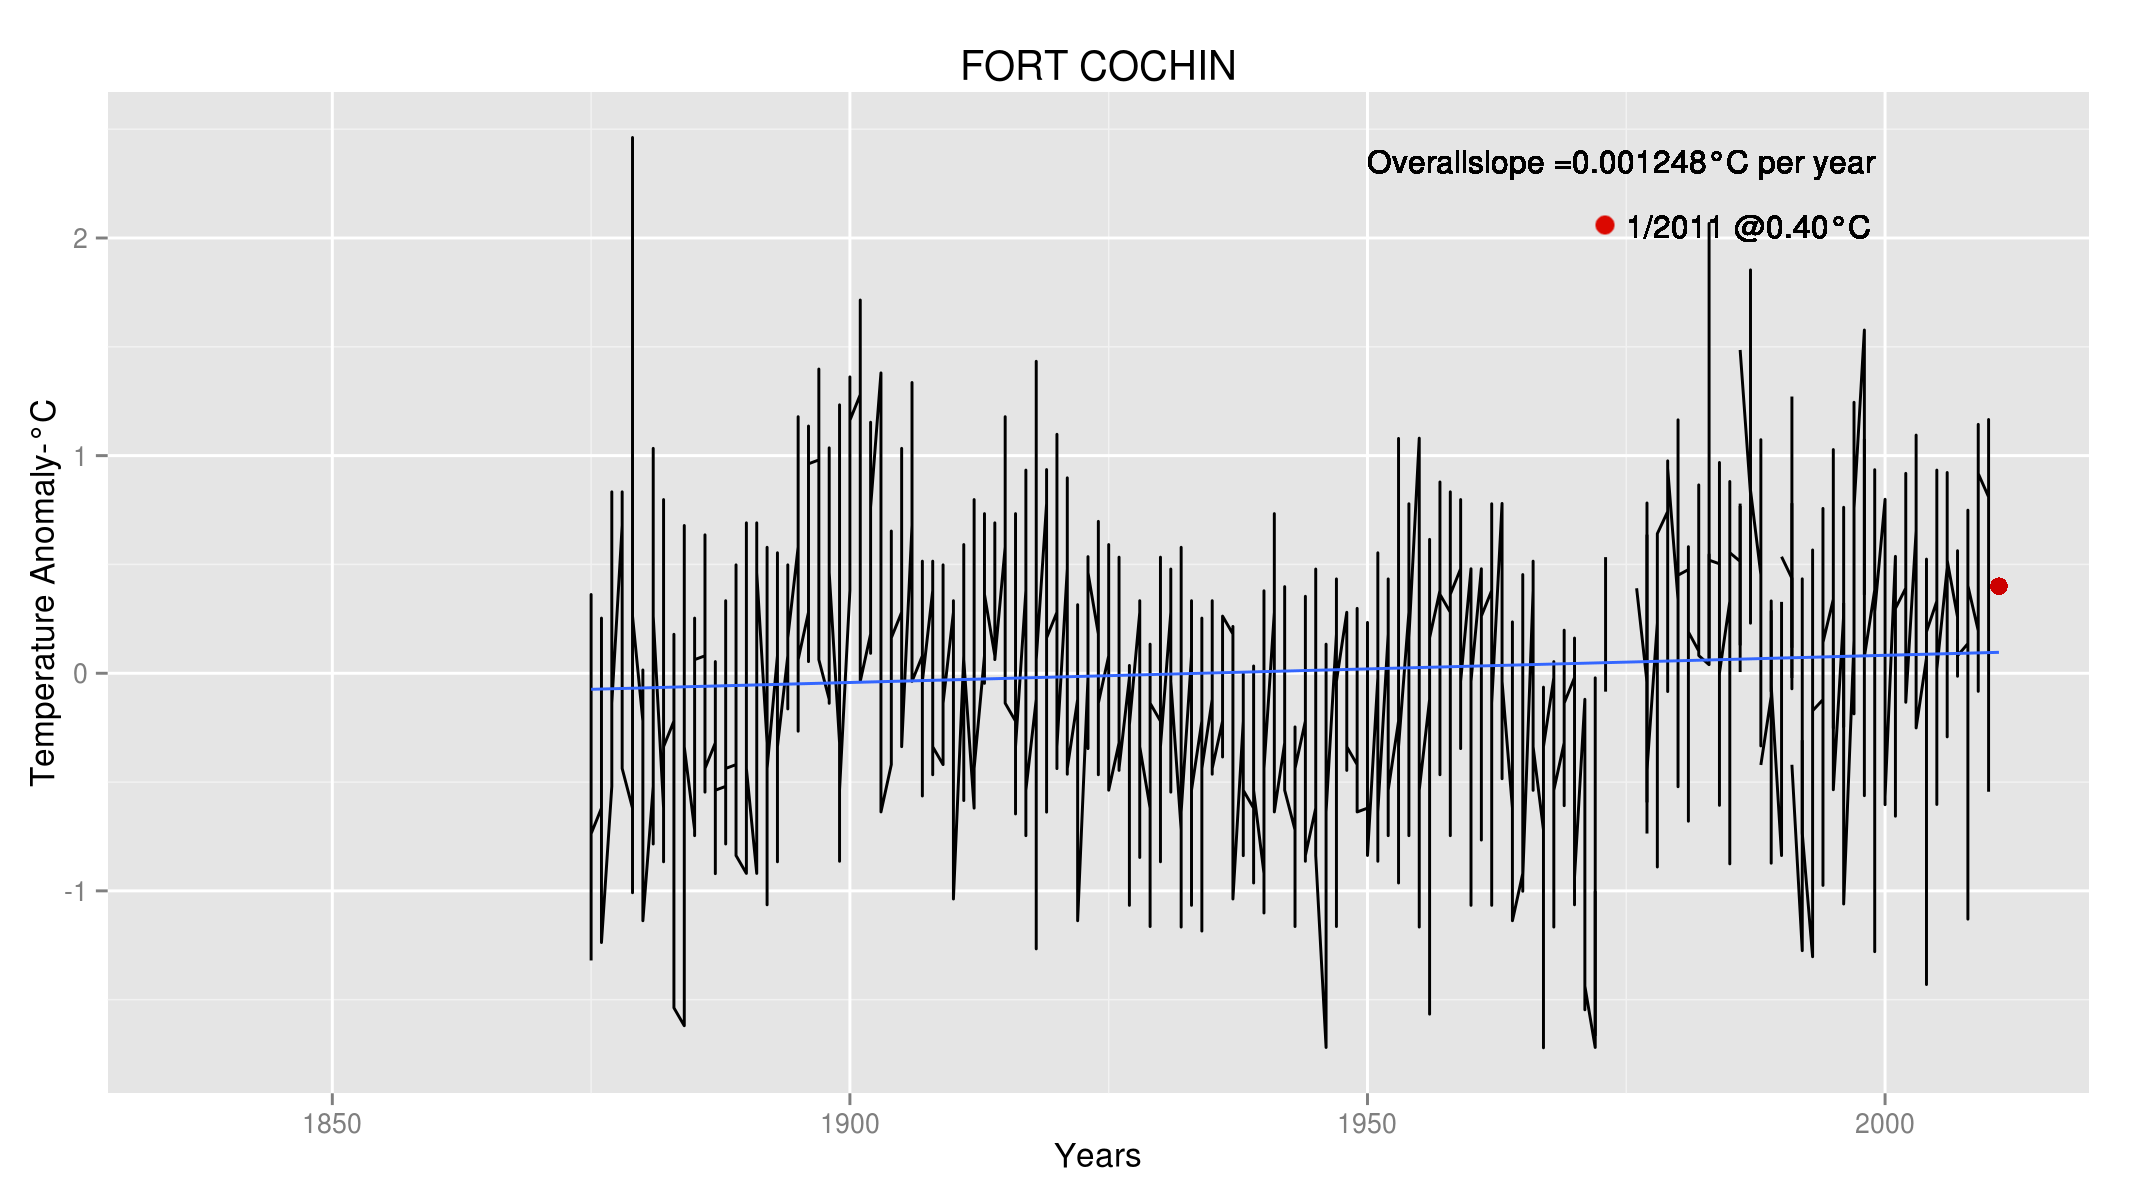
\includegraphics[width=3.2cm,height=3.2cm]{X15079.png}&
	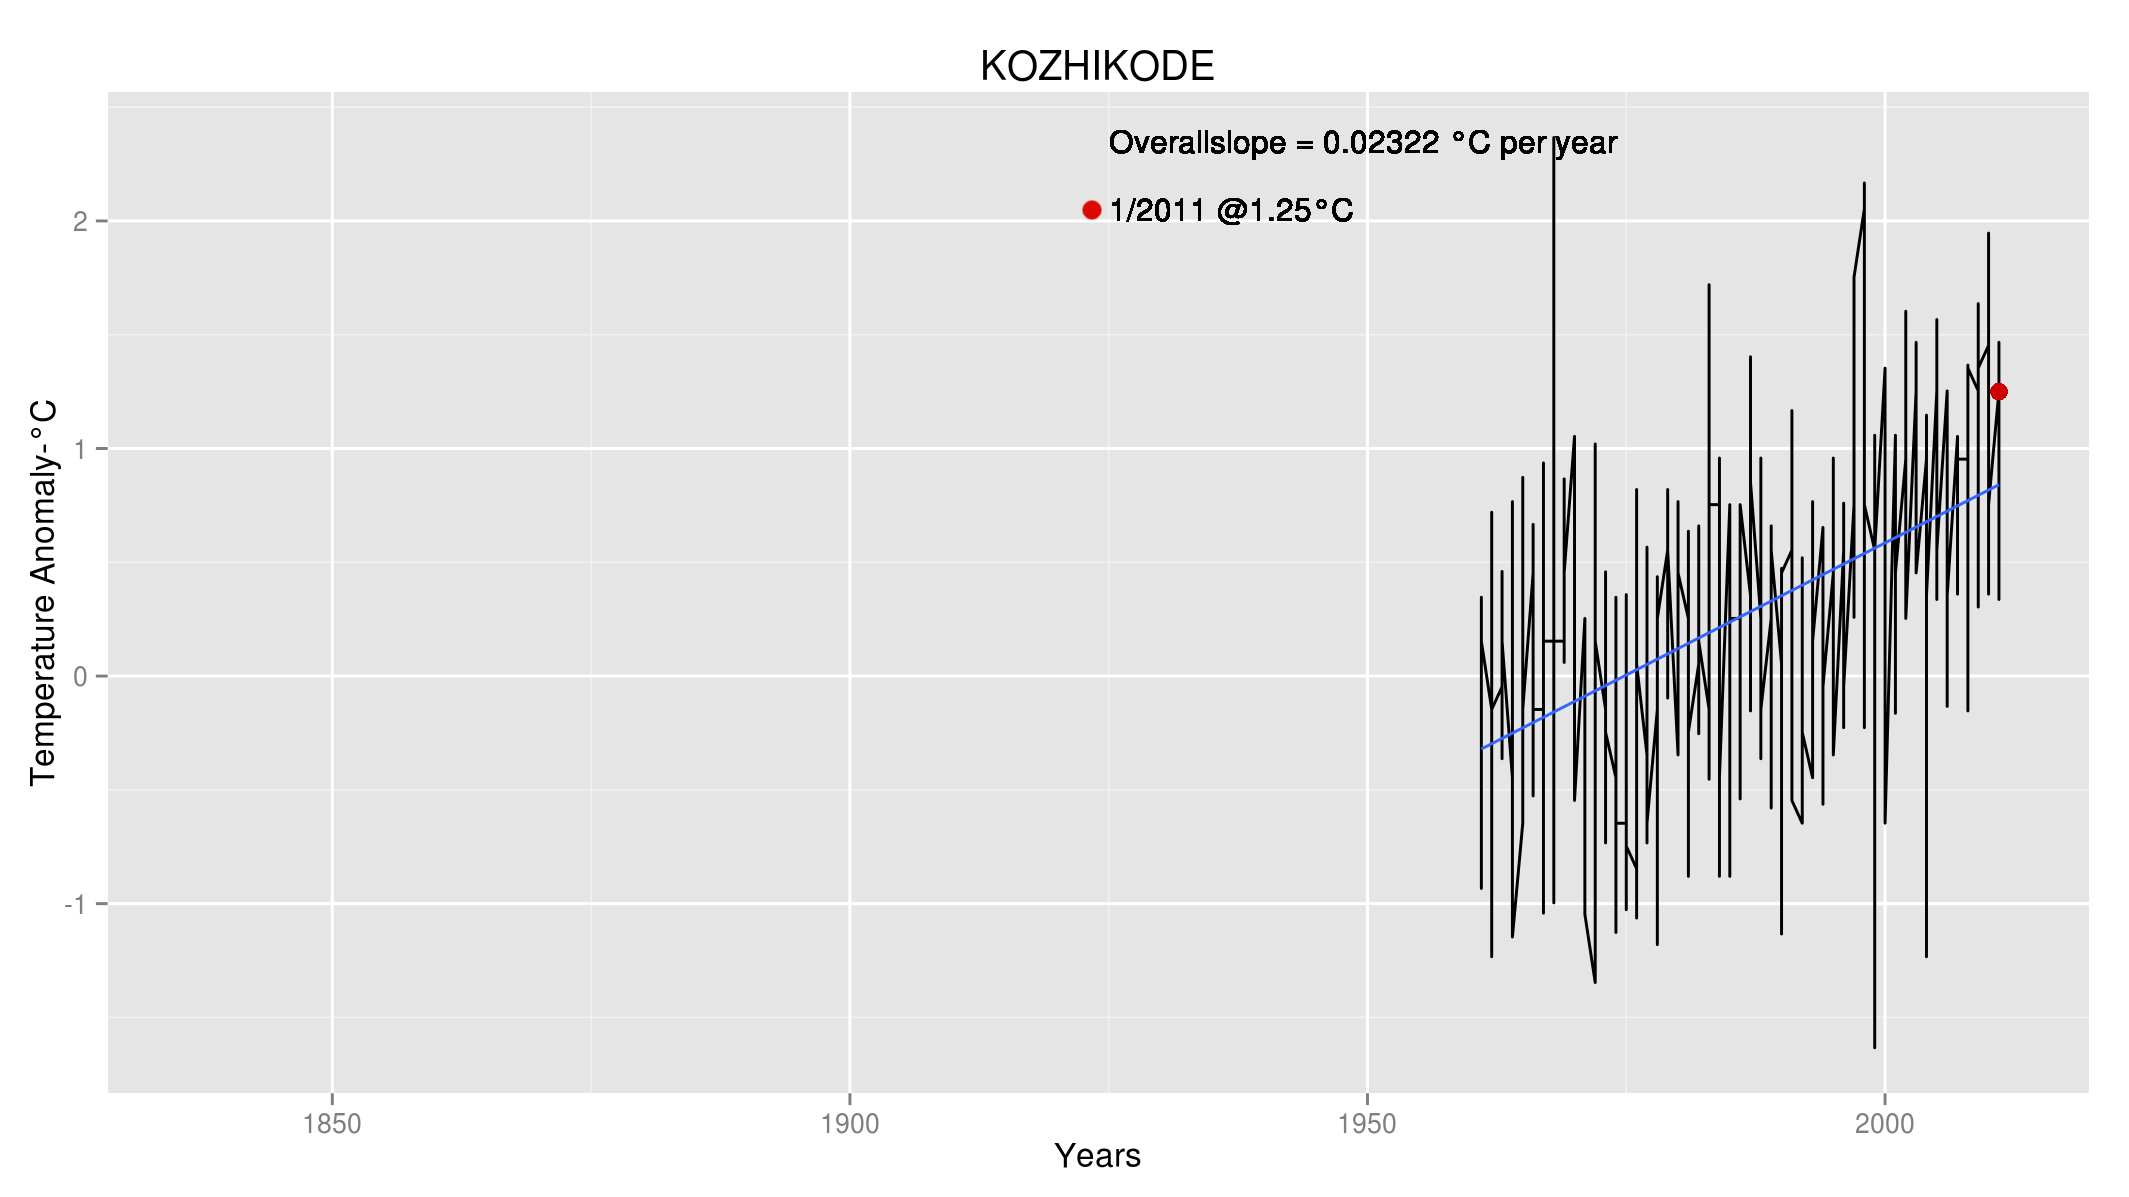
\includegraphics[width=3.2cm,height=3.2cm]{X15088.png}&
	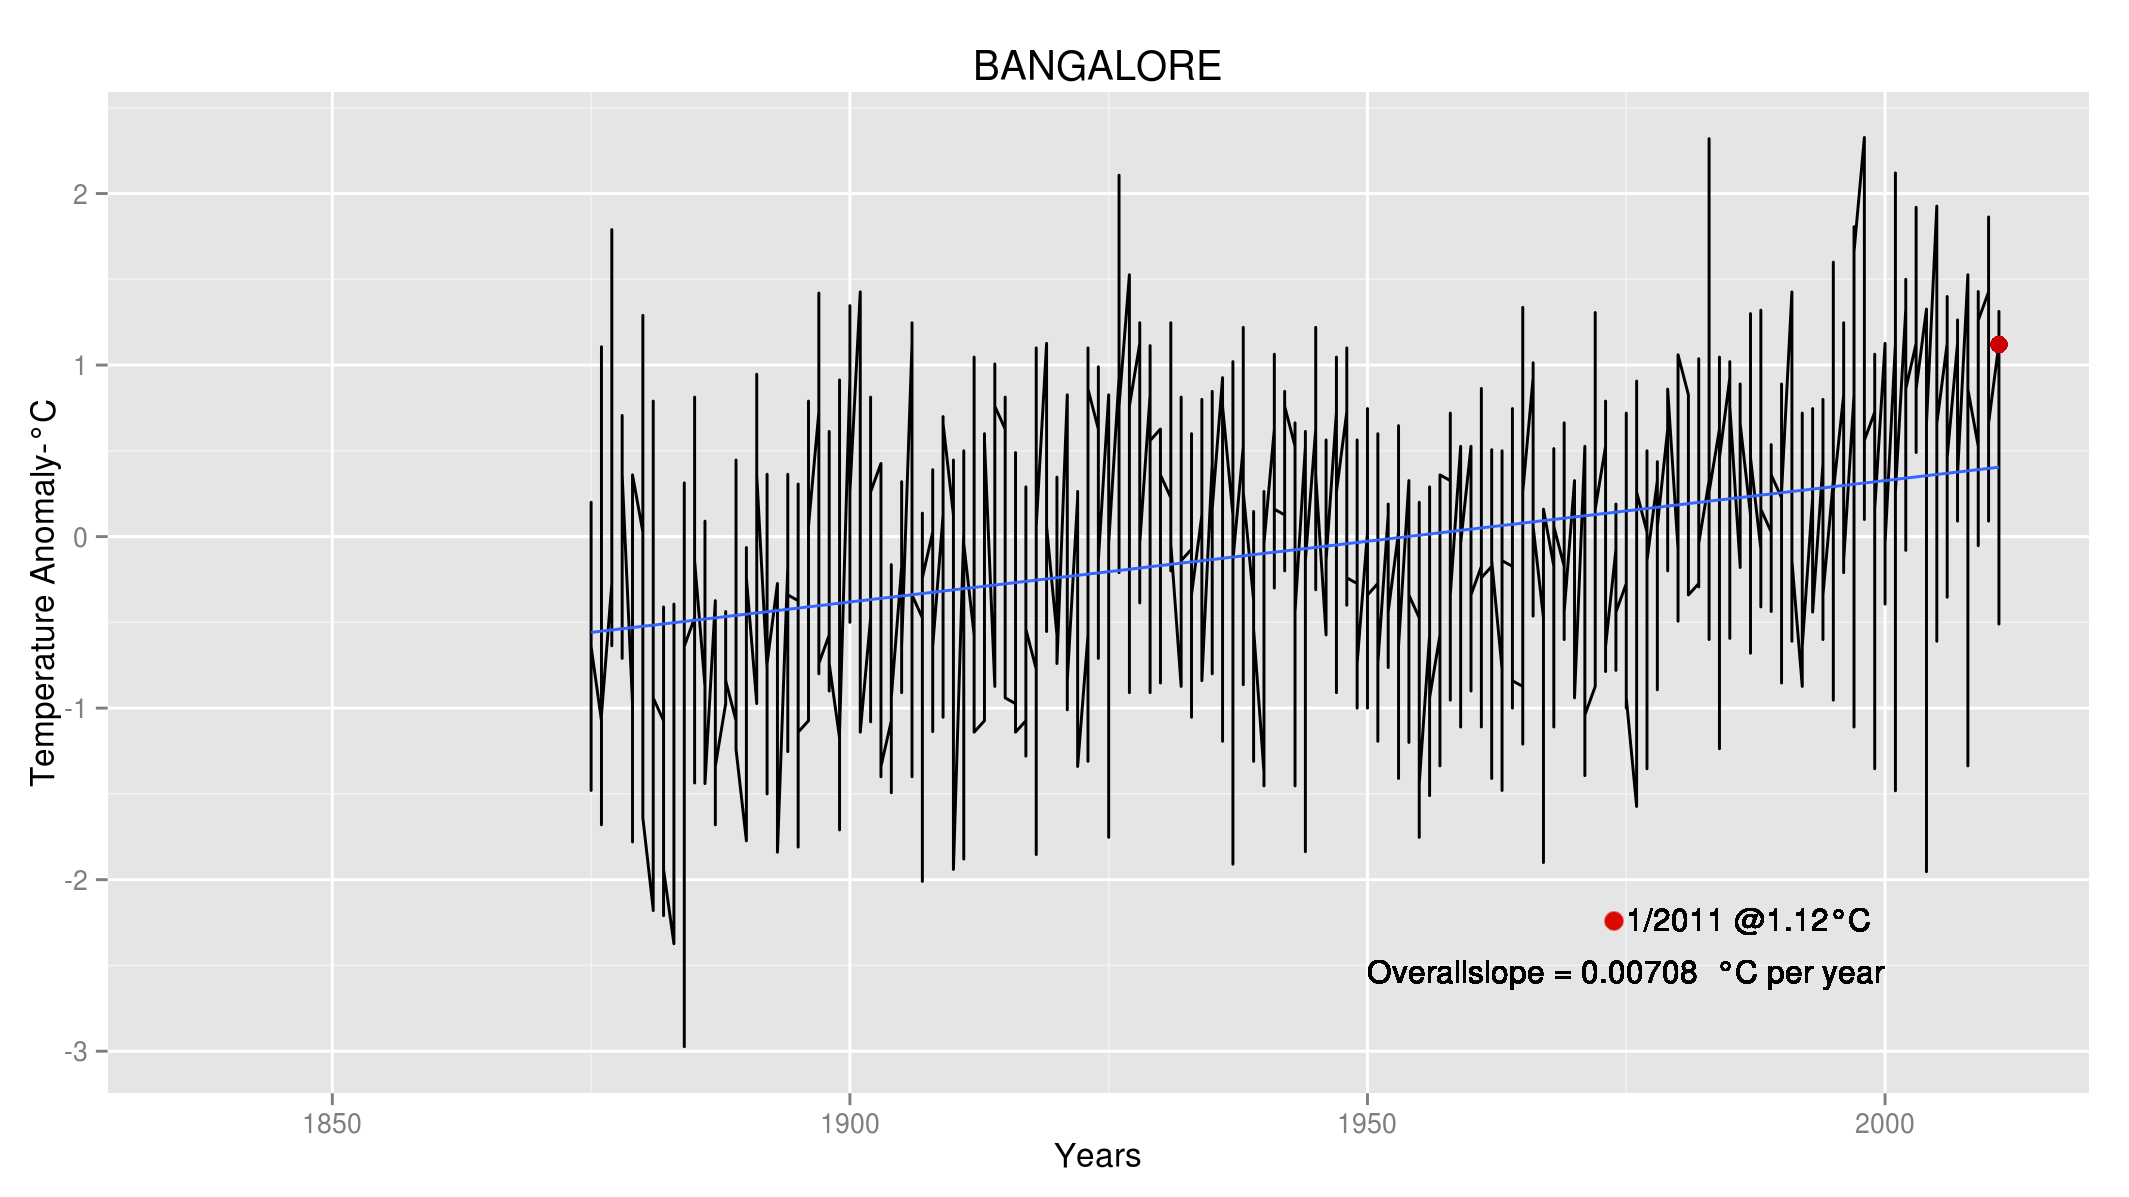
\includegraphics[width=3.2cm,height=3.2cm]{X15098.png}&
	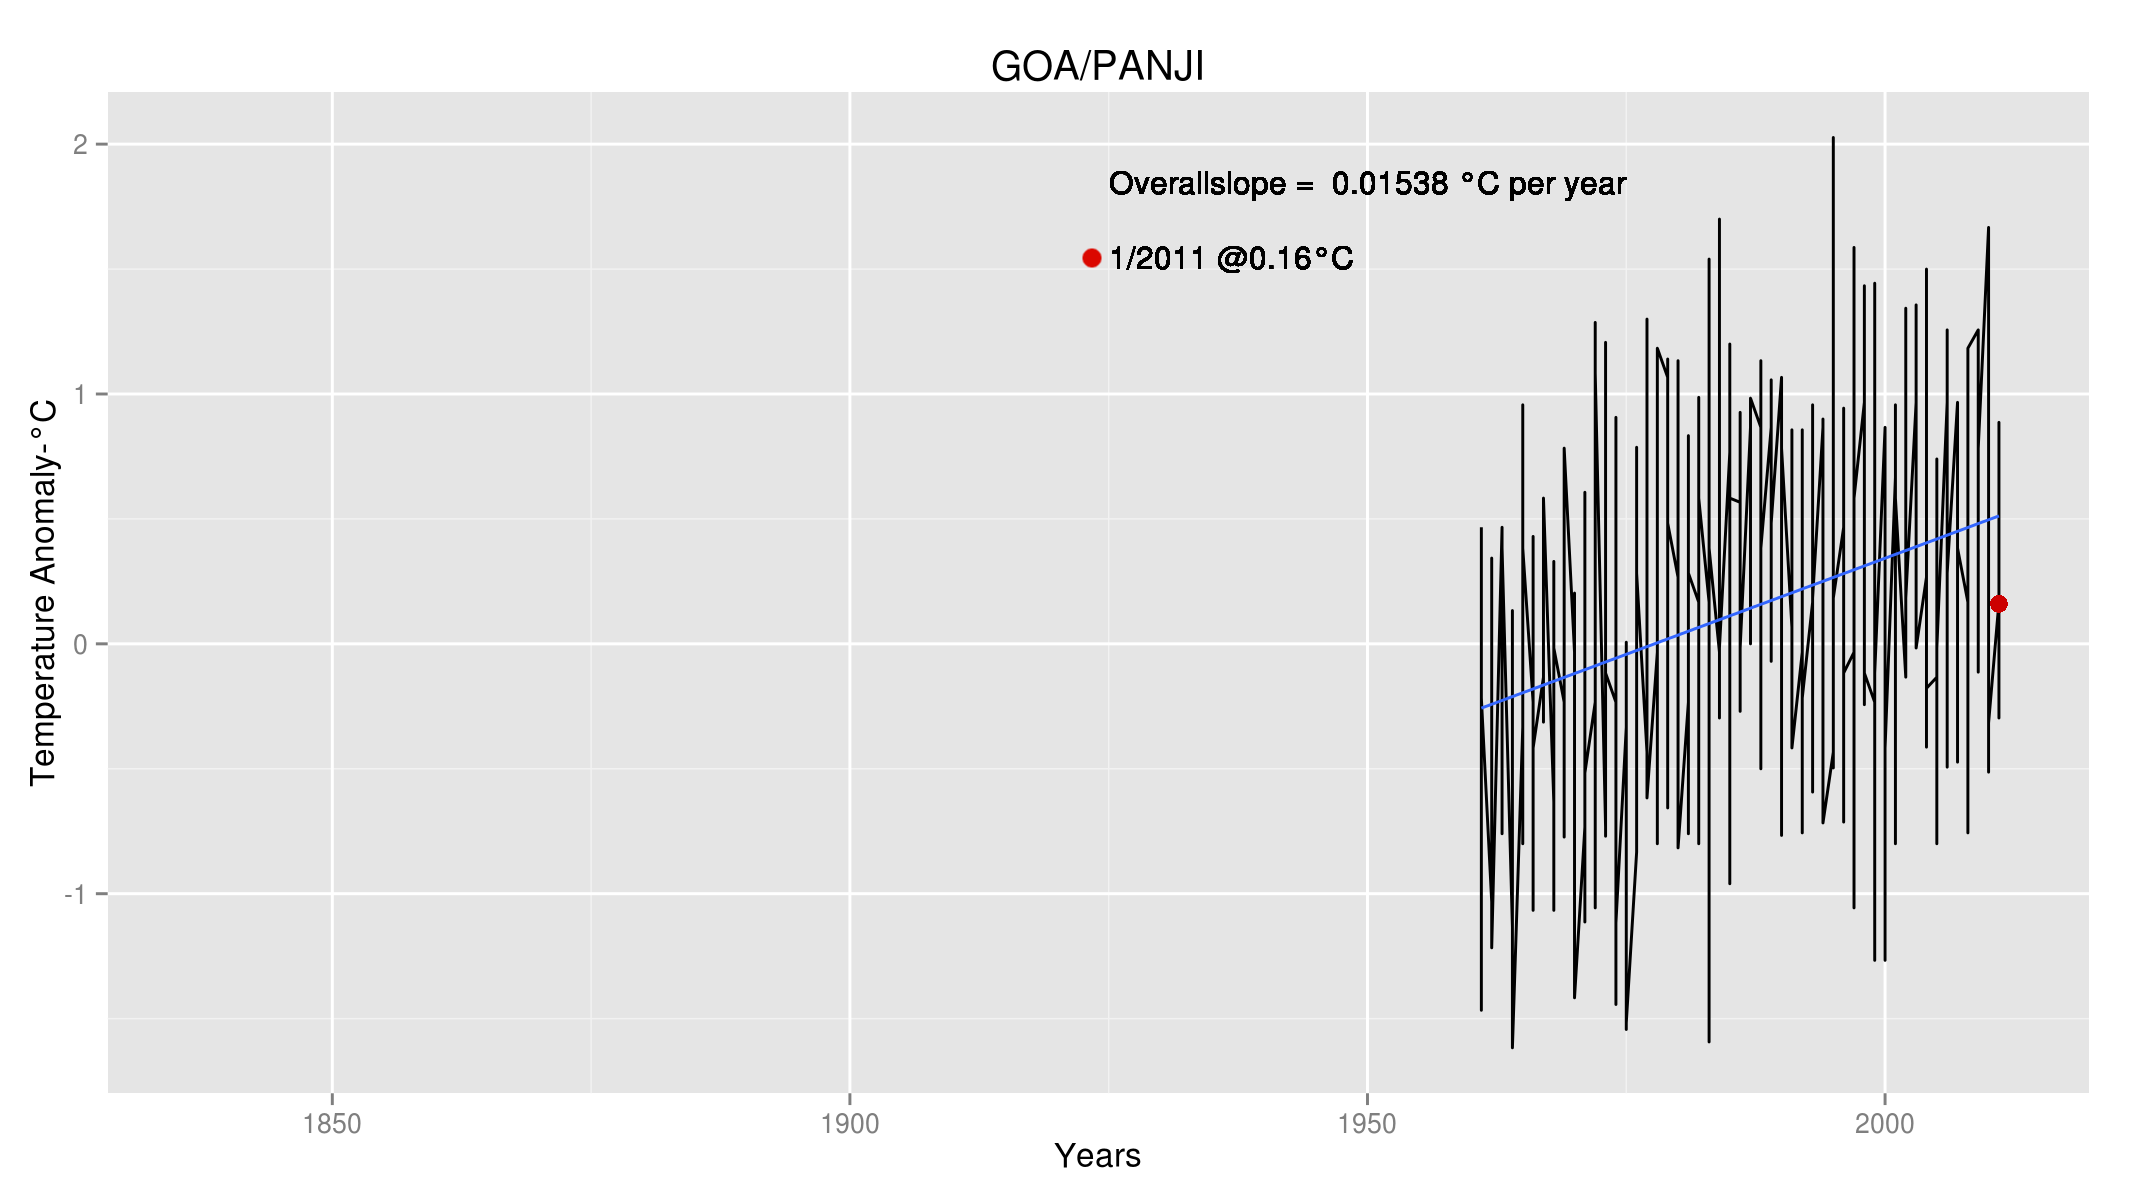
\includegraphics[width=3.2cm,height=3.2cm]{X15110.png}&\\
	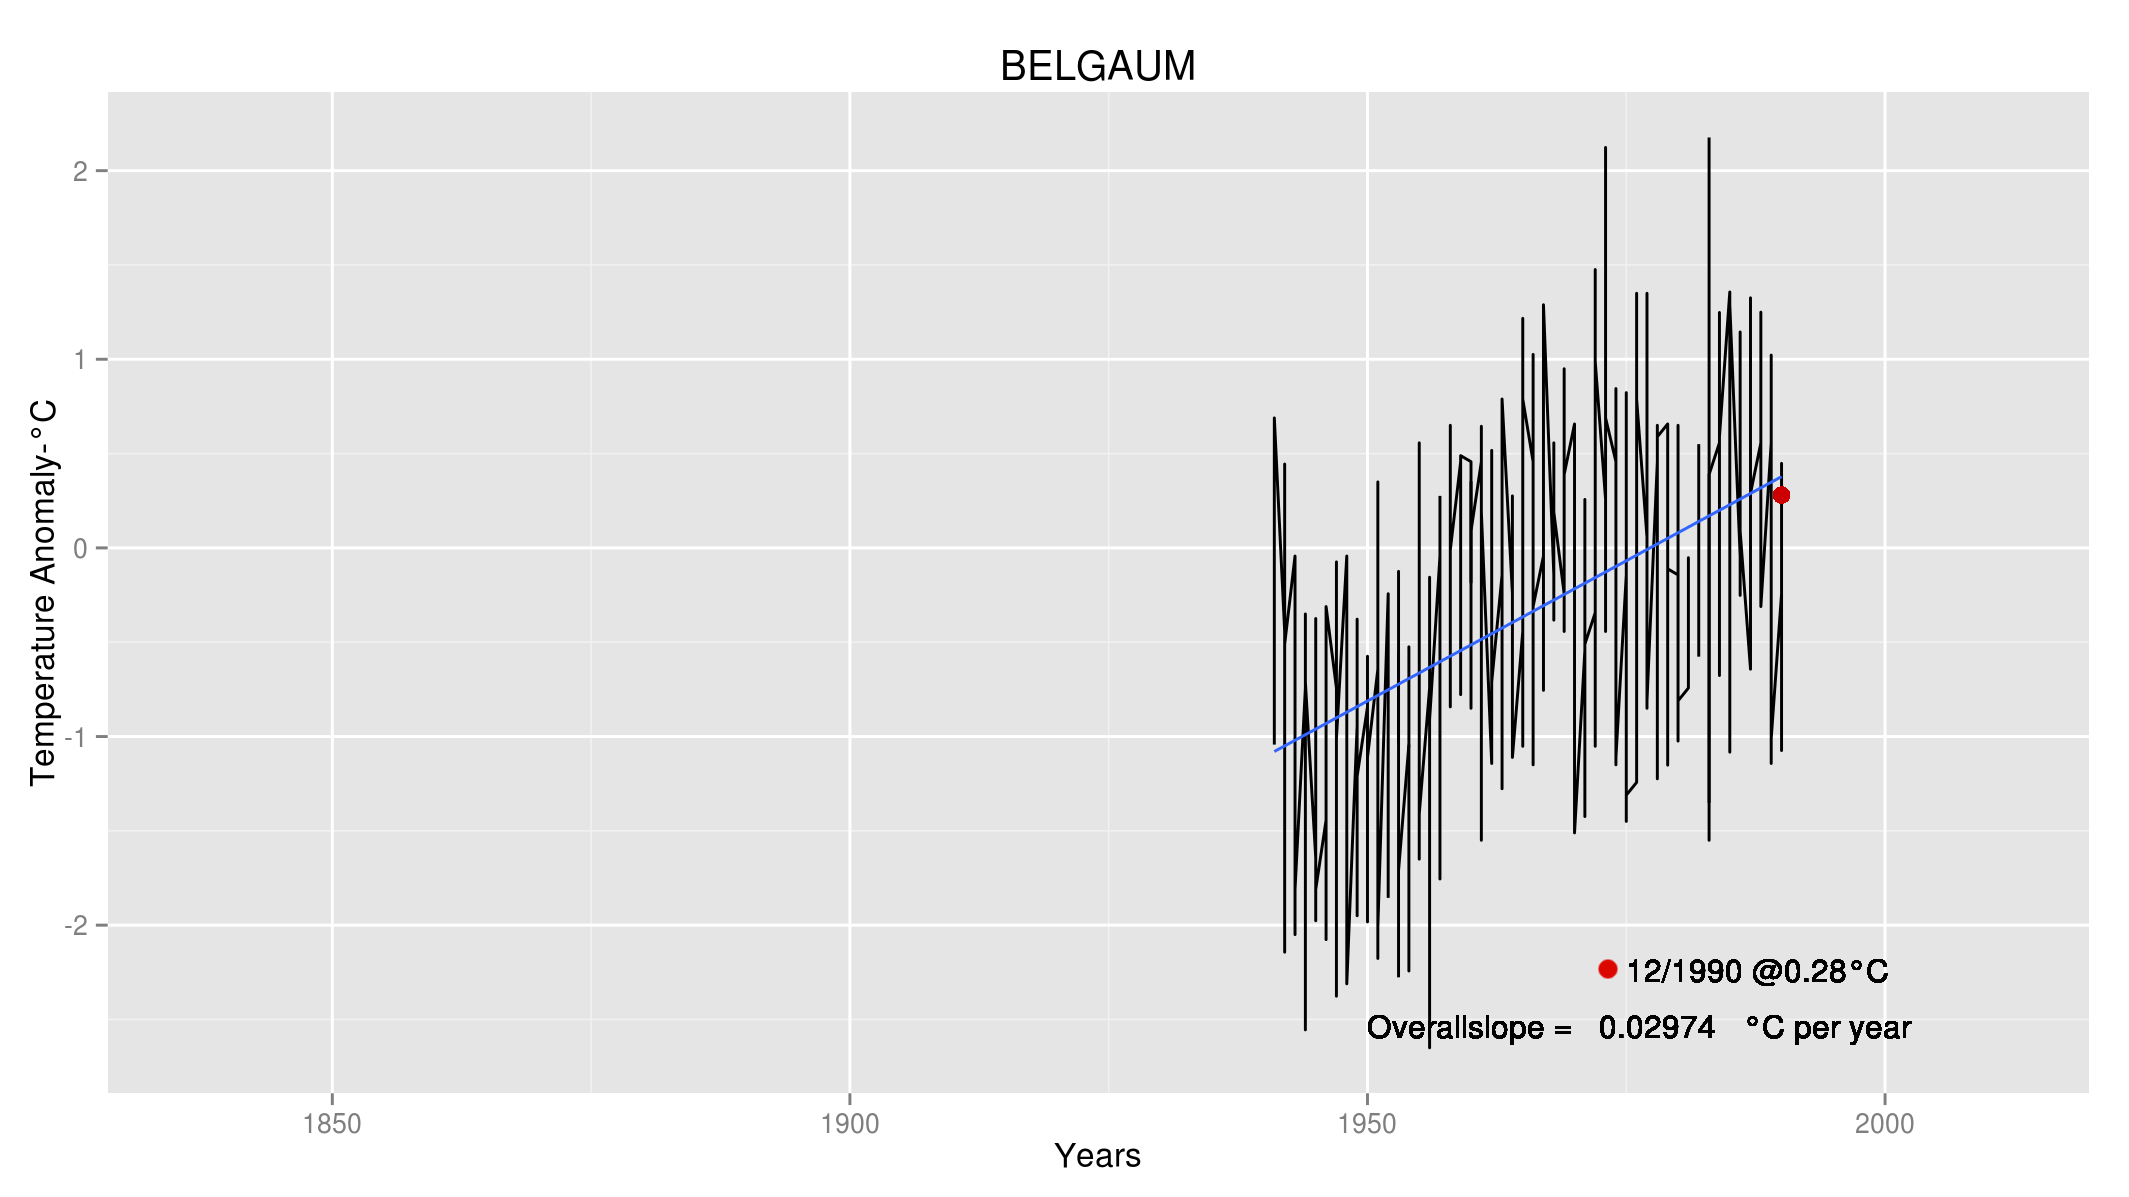
\includegraphics[width=3.2cm,height=3.2cm]{X15113.png}&
	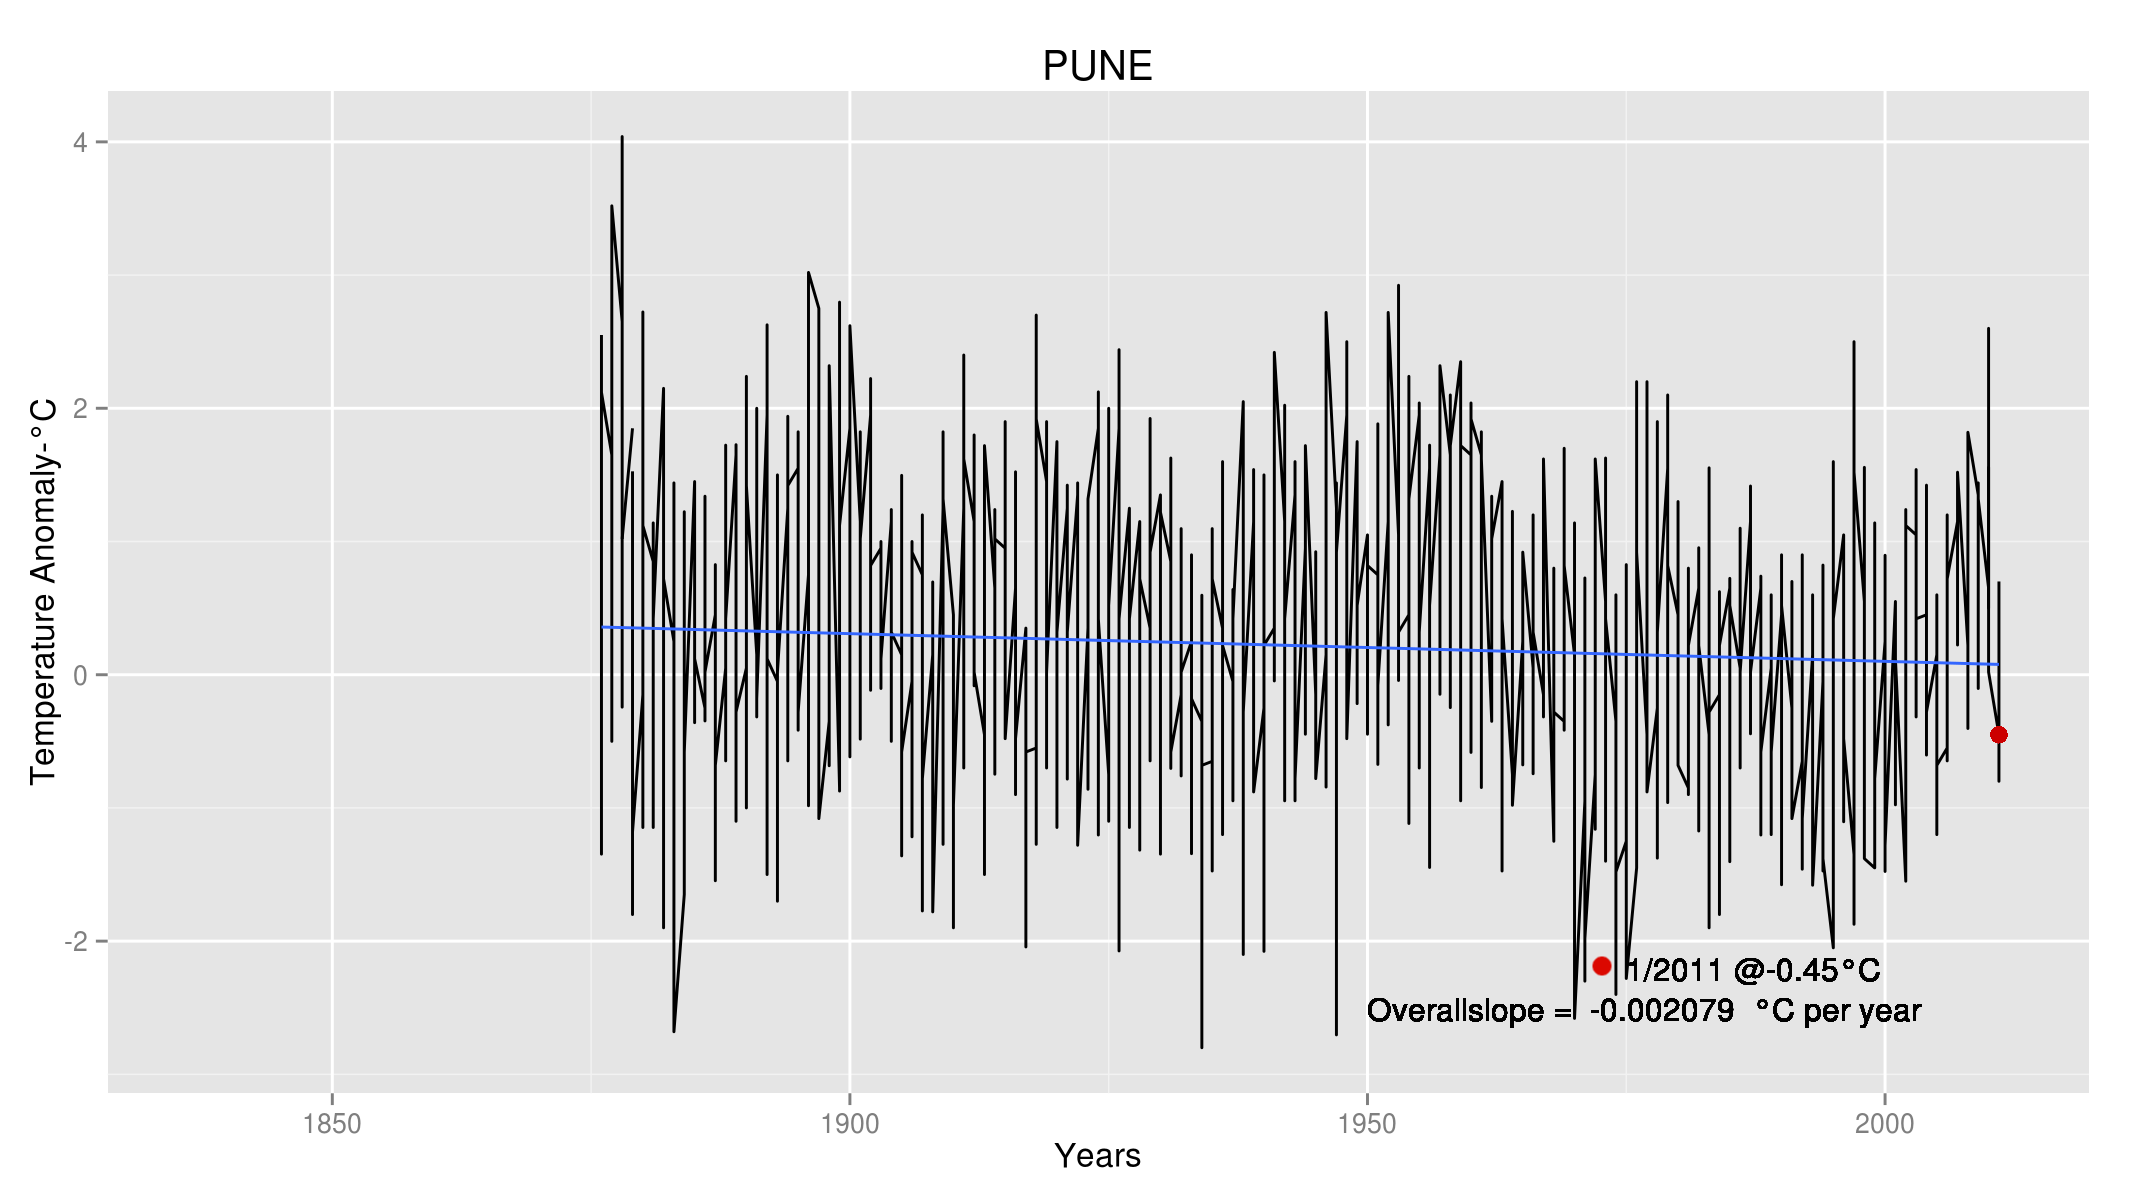
\includegraphics[width=3.2cm,height=3.2cm]{X15130.png}&
	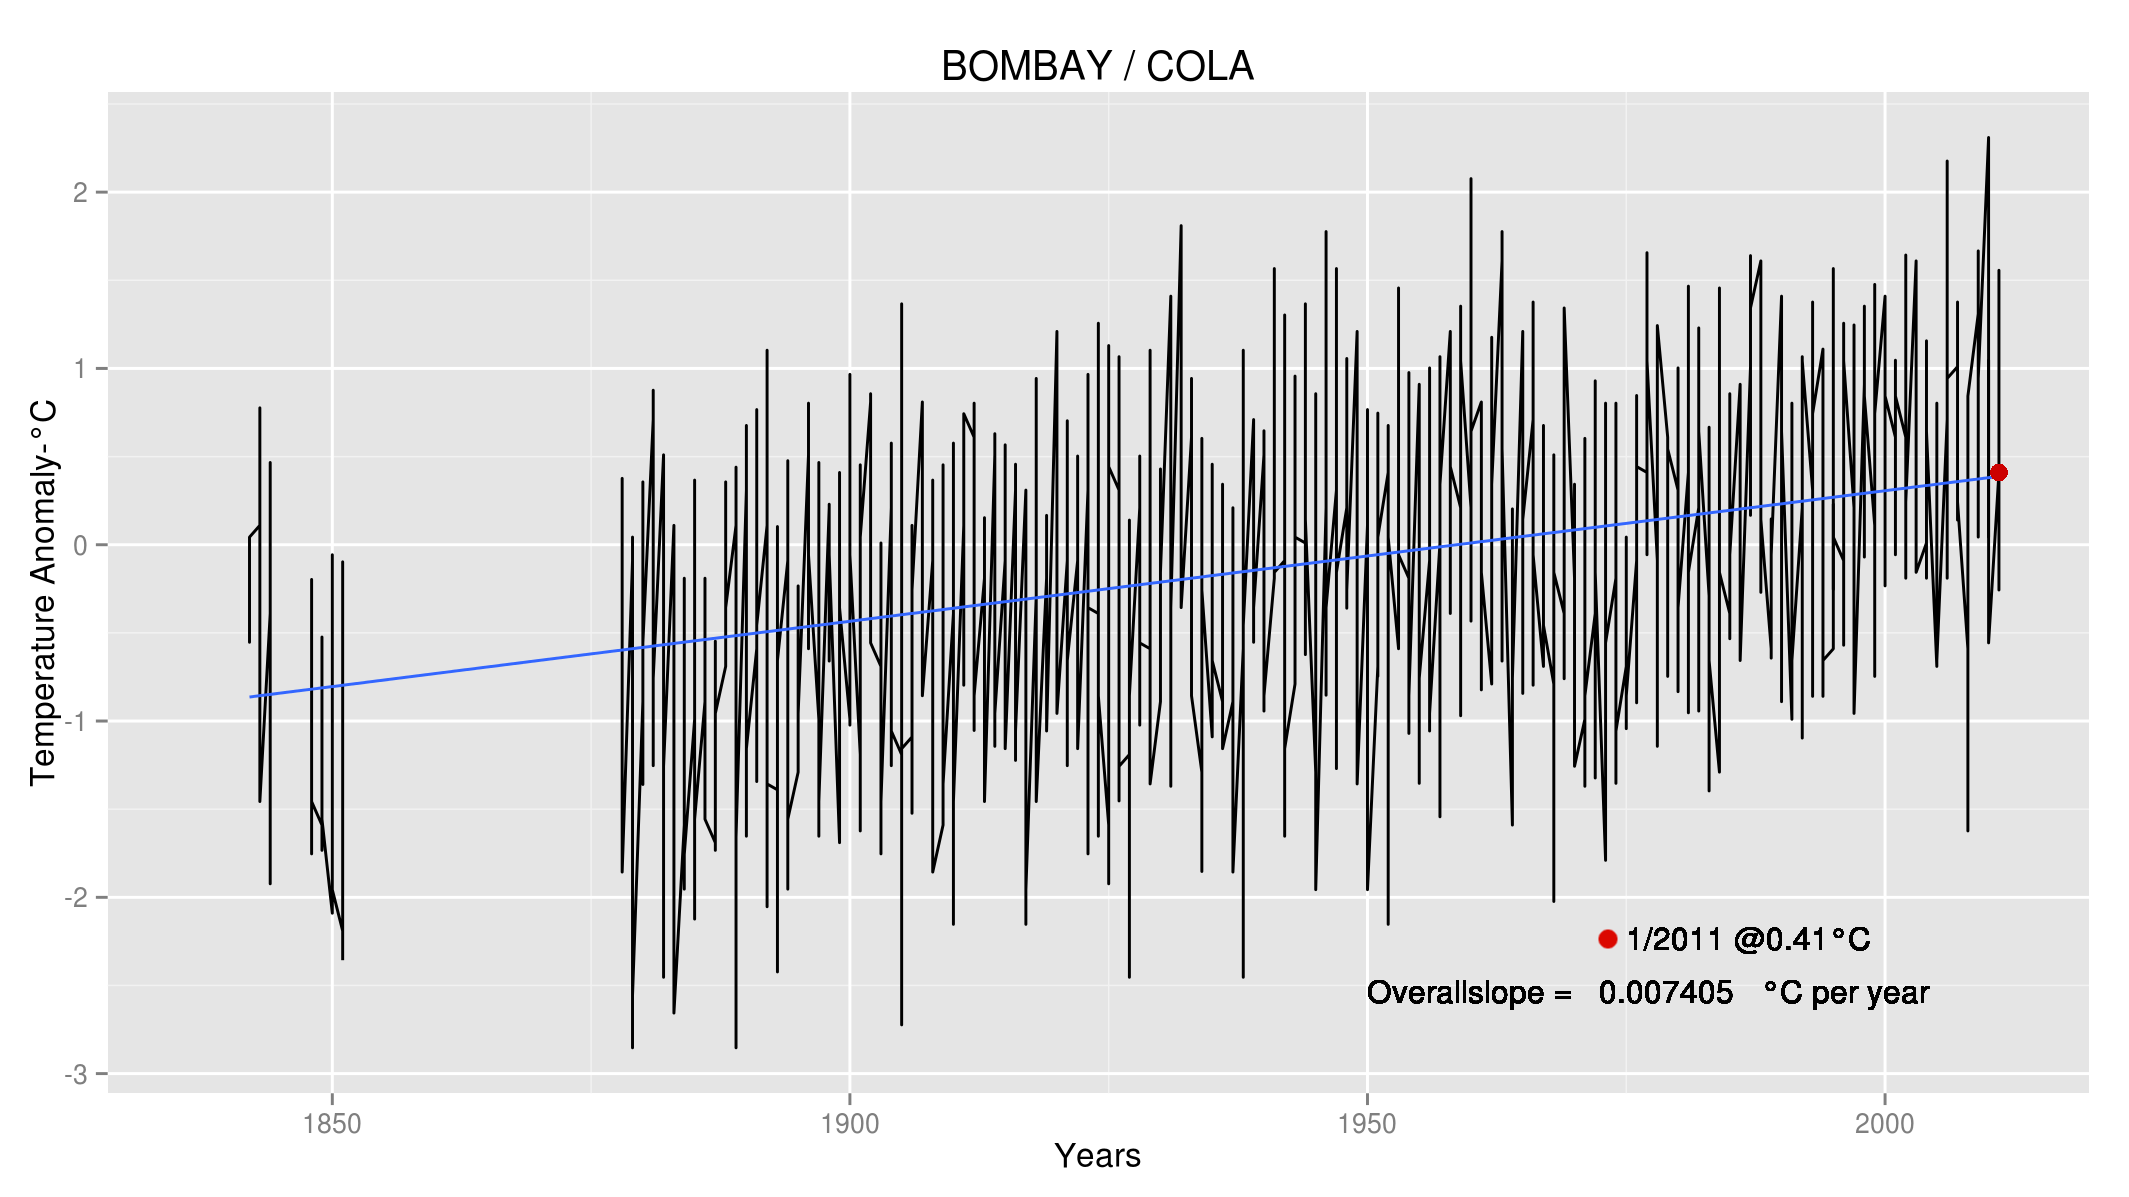
\includegraphics[width=3.2cm,height=3.2cm]{X15133.png}&
	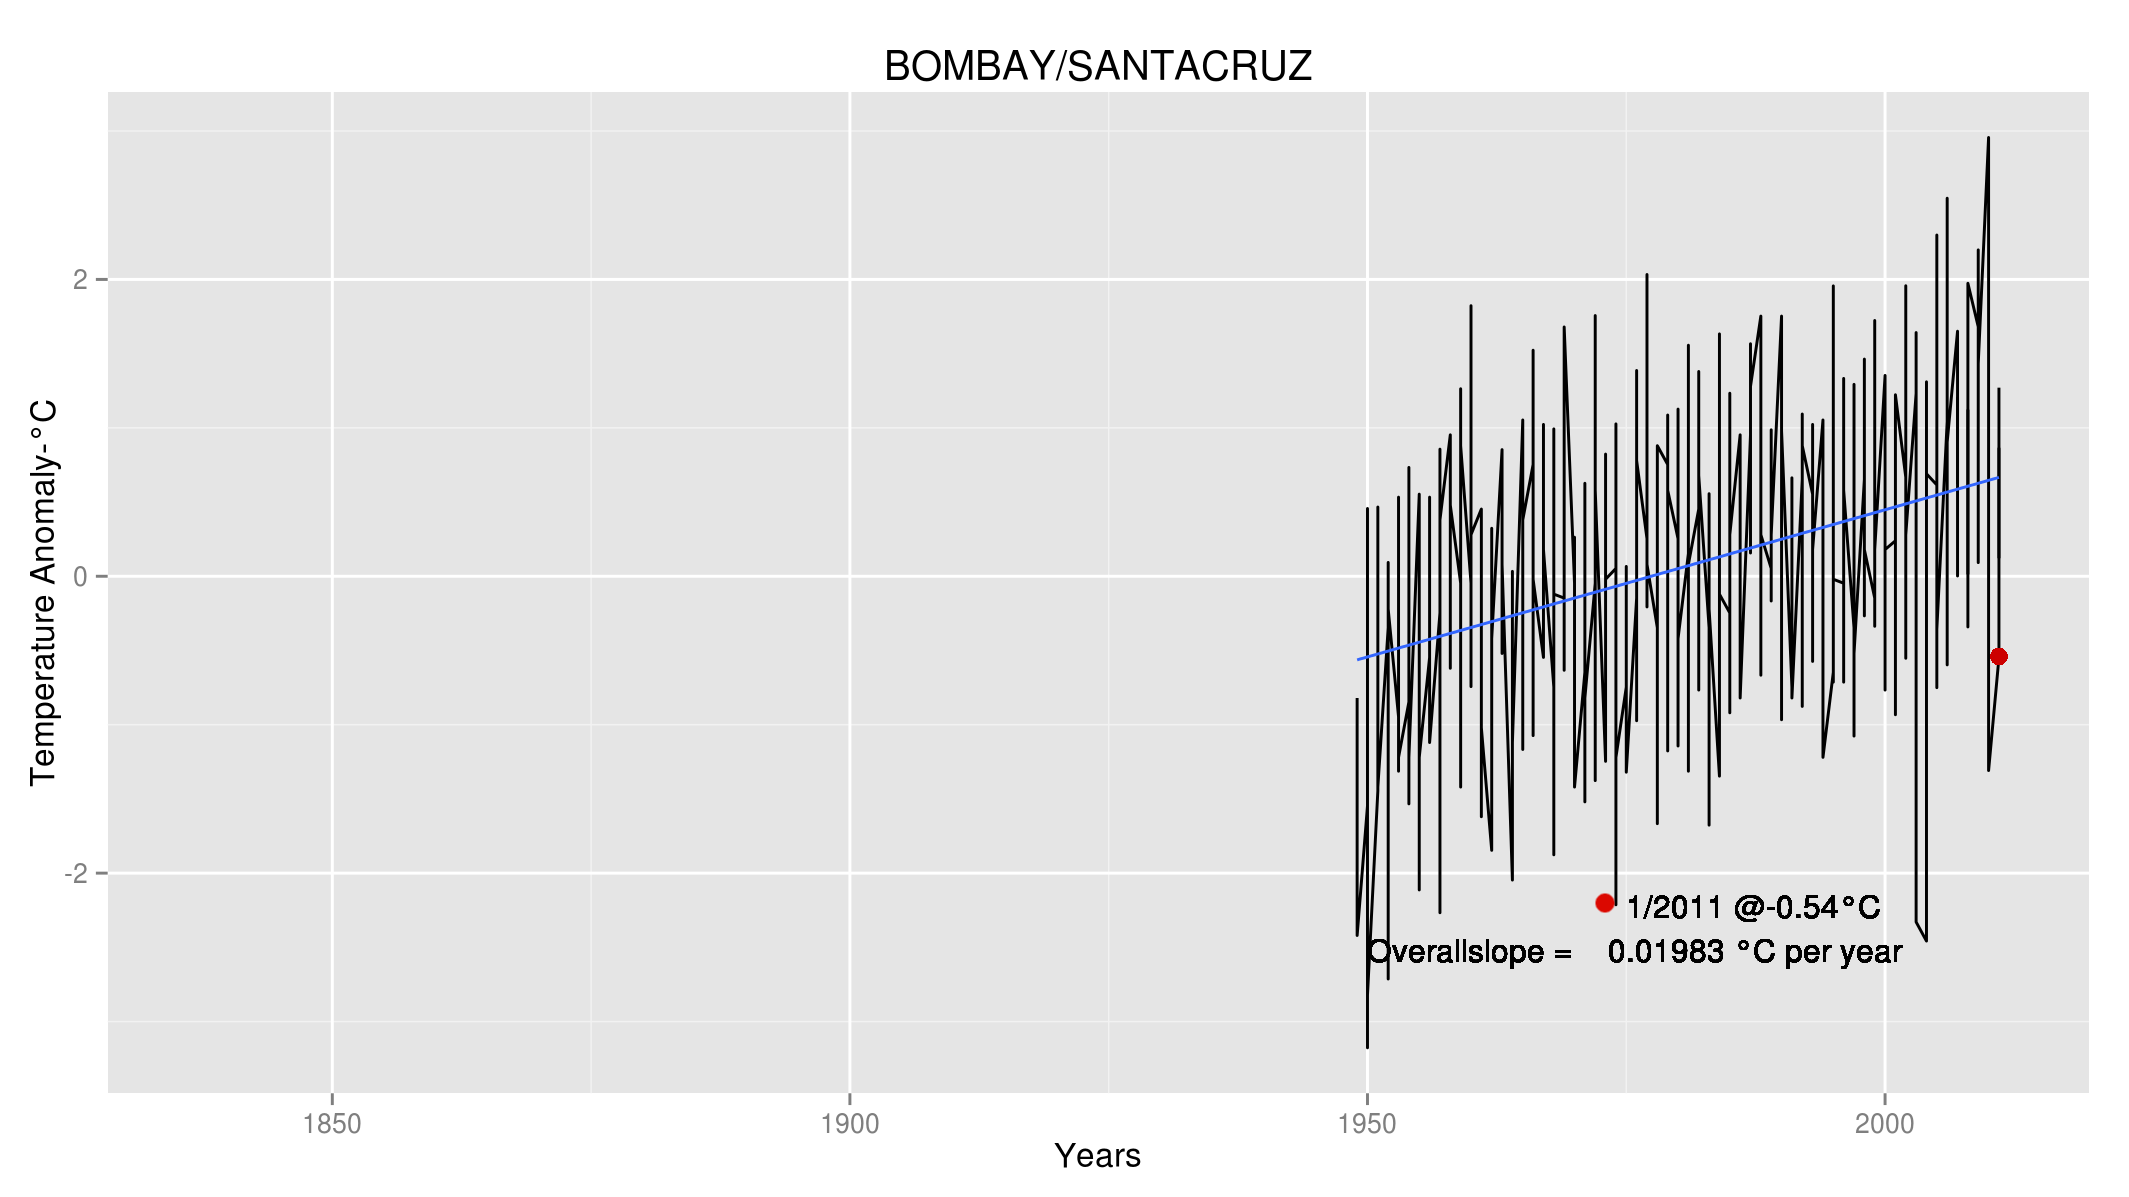
\includegraphics[width=3.2cm,height=3.2cm]{X15135.png}\\
	                       
  \end{tabular}
\captionof{figure}{\scriptsize Temperature anamoly in different stations of the Western Ghats} 
  \end{minipage} 
 \vspace{0.03 cm}
}



%\headerbox{Conclusion}{name=conclusion,column=2,span=2,row=0,below=results1}{
%  %%%%%%%%%%%%%%%%%%%%%%%%%%%%%%%%%%%%%%%%%%%%%%%%%%%%%%%%%%%%%%%%%%%%%%%%%%%%%%
%    
%      \begin{multicols}{2}
%    Between one and three user clicks were needed to achieve accurate tracking for
%      the head sequence. Note the correct handling of the occluded ear, which
%      required only a single click. 
%
%      The eye of the running giraffe required eight user interactions, of which three
%      marked occlusions. 
%      \end{multicols}
%      \vspace{2em}
%}

%%%%%%%%%%%%%%%%%%%%%%%%%%%%%%%%%%%%%%%%%%%%%%%%%%%%%%%%%%%%%%%%%%%%%%%%%%%%%%
  \headerbox{References}{name=references,column=0,below=methods}{
%%%%%%%%%%%%%%%%%%%%%%%%%%%%%%%%%%%%%%%%%%%%%%%%%%%%%%%%%%%%%%%%%%%%%%%%%%%%%%
    \begin {description}
\tiny
\item R. Rohde, J. Curry, D. Groom, R. Jacobsen, R.A. Muller, S Perlmutter, A. Rosenfeld, C. Wickham, and J. Wurtele. Berkeleyearth temperature averaging process. In review
\item X.L.Wang (2008). Accounting for autocorrelation in detecting mean-shifts in climate data series using the penalized maximal t or F test. J. Appl. Meteor. Climatol., 47, 2423-2444
\item Tamino (2011, July 6).Aligning station records [Blog post]. Retrieved from http://tamino.wordpress.com/2011/07/06/aligning-station-records/
\end {description}
   
  }
%%%%%%%%%%%%%%%%%%%%%%%%%%%%%%%%%%%%%%%%%%%%%%%%%%%%%%%%%%%%%%%%%%%%%%%%%%%%%%
  \headerbox{Conclusion}{name=questions,column=1,span=2,aligned=references,below=methods}{
%%%%%%%%%%%%%%%%%%%%%%%%%%%%%%%%%%%%%%%%%%%%%%%%%%%%%%%%%%%%%%%%%%%%%%%%%%%%%%
  \begin {description}
\scriptsize 
\item Significant positive trend in regional average TAVG, TMAX and negative trend in TMIN; but shows site specific variability.
\item The variability needs to be explored further looking at the local landscape and the ongoing landscapes level changes.
\item The level of uncertainty has to be evaluated along with Kriging based interpolationto know about the spatial variability and directionality.
\end {description}
   \vspace{0.1em}
  }
%%%%%%%%%%%%%%%%%%%%%%%%%%%%%%%%%%%%%%%%%%%%%%%%%%%%%%%%%%%%%%%%%%%%%%%%%%%%%%
  \headerbox{Acknowledgement}{name=a
  cknowledgement,column=3,aligned=references,below=results1}{
%%%%%%%%%%%%%%%%%%%%%%%%%%%%%%%%%%%%%%%%%%%%%%%%%%%%%%%%%%%%%%%%%%%%%%%%%%%%%%
 \tiny
We are thank full to all the authors of R packages used in the analysis especially Mr. Steven Mosher. The Berkley Earth study data set was analyzed using BerkleyEarth and RghcnV3 package, Mann Kendall statistics was carried out using Kendal package, the homogeneity test was carried out using Htest R script and the plots was prepared using ggplot2 package.

  }


\end{poster}

\end{document}
